%!TEX program=xelatex
%!TEX program=bibtex
%!TEX program=xelatex
%!TEX program=xelatex
% !Mode:: "TeX:UTF-8"
%\documentclass[master,openany,twoside,a4paper,AutoFakeBold]{sudathesis}
\documentclass[master,openany,twoside,a4paper,AutoFakeBold]{sudathesis}
\usepackage{tikz-dependency}
\usepackage{graphicx}
\usepackage{tikz}
\usepackage{tikz-qtree}
\usepackage{caption}
\usepackage{subcaption}

\usepackage{pgfplots}
\usepackage{color}
\usepackage{dashrule}
%\usepackage{colortbl}
%\usepackage{arydshln}
%\usepackage{multirow}
%\usepackage{multicol}
%\usepackage[SlantFont,BoldFont,CJKchecksingle,CJKnumber]{xeCJK}
%\setmainfont[BoldFont=SimHei ,ItalicFont=KaiTi_GB2312]{SimKai}
%\newcommand\fontnamekai{KaiTi_GB2312}

\usepackage{graphics}
\usepackage{pdfpages}

\begin{document}

% 用户信息
% !Mode:: "TeX:UTF-8"

% 学院中英文名,中文不需要“学院”二字
% 院系英文名可从以下导航页面进入各个学院的主页查看
% http://www.buaa.edu.cn/xyykc/index.htm
\school
{计算机科学与技术学院}{School of XXX}

% 专业中英文名
\major
{计算机科学与技术~~~}{XXXX Engineering}

% 方向中英文名
\direct
{自然语言处理~~}{XXXX Engineering}

% 论文中英文标题
% Research on Chinese Named Entity Recognition With Noise Training Data
\thesistitle
{快速精准的句法分析方法研究}{Research on Fast and Accurate Syntactic Parsing Methods}

% 作者中英文名
\thesisauthor
{张宇~~~~}{Yu Zhang}

% 导师中英文名
\teacher
{李正华}{Zhenghua Li}


% 班级
\class{XXXX}

% 学号
\studentID{20184227035}

% 单位代码
\unicode{10285}

% 论文时间,用于首页
\thesisdate{2021}{3}

%\includepdf{content/mangshen-fengmian.pdf}

% 中英封面、提名页、授权书
\maketitle

% 正文前页码是大写罗马字母
\pagenumbering{Roman}
% 前言页眉页脚样式 % 摘要
\pagestyle{cnfrontmatter}
% !Mode:: "TeX:UTF-8"

% 中英文摘要
\begin{cabstract}
	句法分析任务是句子理解的重要中间过程之一.
	其中,概率估计一直是句法分析领域的一个核心问题.
	然而,无论是神经网络方法还是深度学习时代以前的方法,采用基于全局概率模型的句法分析工作都非常少,主要的原因在于树形条件随机场(TreeCRF)推断的高复杂度.
	在本文中,我们提出将TreeCRF应用到依存句法和成分句法这两个主要的句法分析任务.
	为了解决TreeCRF的低效问题,关键的想法是批次化树结构的推断算法,并且用基于自动求导的反向传播代替Outside算法.
	目前句法模型被不断简化,采用局部损失目标是当前句法分析方法的一个趋势,我们则进一步在一阶TreeCRF的基础上采用了高阶拓展.
	高阶TreeCRF进一步增加了算法复杂度,为此,我们还提出利用基于平均场变分推断的近似推断算法代替精确推断的TreeCRF方法,从而增加了解析效率.

	具体而言,本文的研究内容主要包含三个方面:
	\begin{enumerate}

		\item 基于TreeCRF的高阶依存句法分析方法

		      本文提出将TreeCRF方法应用到神经依存句法分析器当中,并进一步提出了一个二阶TreeCRF的扩展.
		      导致TreeCRF低效的主要瓶颈在于Inside-Outside算法,尤其是Outside算法的计算.
		      为了解决这个问题,一方面,我们提出对Inside算法进行批次化,从而利用GPU的并行计算能力来加速,将算法复杂度从$O(n^3)$降低到了$O(n^2)$.
		      另一方面,我们还提出将复杂的Outside算法用高效的反向传播代替,显著提升了效率,使得一阶和二阶模型的速度分别达到了500和400句每秒.
		      我们在13个语言的27个数据集上进行了详细实验,结果表明了TreeCRF和高阶建模的有效性.

		\item 基于TreeCRF的高阶成分句法分析方法

		      本文提出将高阶TreeCRF应用到成分句法分析中.
		      为了解决效率问题,我们应用了和依存模型中一致的批次化技术和反向传播来加速.
		      此外,我们提出一个简单的两阶段解析方法,和前人的一阶段解析相比结果相当,但是更加高效.
		      我们还参考了依存句法的模型架构和参数设置,提出用双仿射打分机制替换传统打分方法,发现在双向LSTM编码器中引入的诸如Dropout的策略改进可以极大提升解析的性能.
		      在中英文三个基准数据集上的实验结果表明,我们提出的模型结果显著超越了现有方法,并且一阶和二阶模型的速度分别达到了1,092和598句每秒.
		      我们的模型在使用BERT之后达到了现有最好的结果.

		\item 基于变分推断的高效句法分析方法

		      为了解决精确推断的TreeCRF方法高复杂度的问题,本文提出在依存句法和成分句法分析中引入基于平均场变分推断的近似方法.
		      相比于高阶TreeCRF方法,变分推断将算法在GPU上的复杂度从$O(n^2)$降低到了$O(n)$,大大提升了模型效率.
		      在中英文共五个数据集上的实验结果表明,我们的二阶变分推断方法在性能上显著超越了一阶模型,达到了和二阶TreeCRF模型可比较的水平,与此同时在依存句法和成分句法上的解析速度分别达到了1,126句每秒和905句每秒,大大超越了精确推断的二阶TreeCRF.
		      此外,使用BERT之后,我们的变分推断方法的结果达到或接近了现有的最佳结果.

	\end{enumerate}

	综上,我们在依存和成分句法这两种句法分析任务上提出应用TreeCRF以及一个二阶TreeCRF拓展,显著提升了句法分析器的性能.
	我们采用批次化以及反向传播等加速技术,解决了TreeCRF的效率问题.
	本文同样还探究了变分法等近似方法对解析效率的影响.
	我们发现变分法在保持高阶模型的性能的同时,大大加快了解析速度.

	\vskip 21bp
		{\heiti\zihao{-4} 关键词:}
	句法分析,
	依存句法分析,
	成分句法分析,
	树形条件随机场,
	变分推断

	\begin{flushright}
		作~~~~~~~~者:***

		指导老师:***

	\end{flushright}
\end{cabstract}




\pagestyle{enfrontmatter}
% !Mode:: "TeX:UTF-8"

\begin{eabstract}
	Syntactic parsing is one of the most important intermediate processes of sentence comprehension.
	However, in both deep learning (DL) and pre-DL eras, very few works have adopted global probabilistic models, mainly due to the high complexity of probabilistic inference algorithm for syntax trees.
	In this thesis, we propose to apply TreeCRF to dependency and constituency parsing.
	Compared with previous works, the advantage of TreeCRF is to obtain tree/subtree probabilities, which is more useful for downstream tasks.
	The main bottleneck leading to the inefficiency of TreeCRF lies in the Inside-Outside algorithm, especially the calculation of the Outside pass.
	To solve this, on the one hand, we propose to batchify the Inside algorithm, so as to utilize the parallel computing power of GPU to speed up.
	On the other hand, we also propose to replace the complex Outside algorithm with efficient back-propagation.
	In deep learning era, models are greatly simplified.
	It's a trend to adopt local loss (classification) for both dependency and constituency parsing.
	We propose a high-order extension based on the first-order TreeCRF.
	High order modeling further increases the time complexity.
	To this end, we also try to apply the approximate mean field variational inference algorithm as an alternative to exact inference of TreeCRF method, improving the parsing efficiency greatly.
	We conduct experiments on several benchmark datasets of dependency and constituency parsing, and find that exact inference of high-order TreeCRF brings significant improvement.
	The proposed variational inference method achieves or approaches the performance of high-order TreeCRF method, and greatly improves the parsing speed.
	
	Overall, the main research content of this thesis includes three aspects:
	
	\begin{enumerate}
		\item We propose a TreeCRF-based high-order method for dependency parsing.
		      This thesis proposes a second-order TreeCRF extension to Biaffine Parser that adopts a local training objective, and uses adjacent sibling subtrees as second-order features.
		      To integrate second-order subtree scores more effectively, inspired by biaffine scorer, we propose a novel triaffine structure for scoring.
		      Second-order TreeCRF method causes severe efficiency issues.
		      To overcome this, we propose to batchify the Inside algorithm and use the GPU parallel computing ability to reduce the time complexity from $O(n^3)$ to $O(n^2)$.
		      In addition, we replace the complex Outside algorithm with back-propagation based on auto-differentiation, which significantly improves the efficiency and speed up the model to 400 sentences/s.
		      We conduct extensive experiments on 27 datasets in 13 languages.
		      Results show that second-order models lead to better convergence performance, perform well on global metrics, and is especially useful for partially annotated data.
		\item We propose a TreeCRF-based high-order method for constituency parsing.
		      This thesis proposes to apply high-order TreeCRF to constituency parsing.
		      To solve the efficiency issue, we apply batchification techniques and back-propagation consistent with the dependency model to accelerate.
		      Moreover, we propose a simple two-stage parsing approach, which has comparable results with previous one-stage methods, but is more efficient.
		      We also refer to the model architecture and parameter settings of dependency models, and propose to replace the traditional scoring method with a biaffine scoring mechanism.
		      We find that the parsing performance can be largely improved via better encoder settings like Dropout configuration, leading to similar results with current state-of-the-art Transformer encoder.
		      Experimental results on three Chinese and English benchmark datasets show that our proposed models significantly surpass existing methods.
		      In terms of parsing speed, our first-order and second-order models can parse over 1,092/598 sentences/s.
		      After using BERT, our models achieve new state-of-the-art performance on all datasets.
		\item We propose an efficient syntactic parsing method based on variational inference.
		      In order to deal with the high complexity of the TreeCRF method for exact inference, this thesis proposes to introduce an approximate method based on mean field variational inference for dependency and constituency parsing.
		      Compared with high-order TreeCRF, variational inference reduces the time complexity on GPU from $O(n^2)$ to $O(n)$, improving the model efficiency greatly.
		      We design different factor graphs and corresponding variational inference updating algorithms for dependency and constituency parsing.
		      Experimental results on five Chinese and English datasets show that our second-order variational inference method significantly outperforms the first-order model, and achieves comparable results with second-order TreeCRF models.
		      Meanwhile, our models can parse over 1,126 and 905 sentences/s on dependency parsing and constituency parsing respectively, greatly surpassing the exact inference of second-order TreeCRF methods .
		      Moreover, after using BERT, our variational inference method achieves or approaches the performance of current state-of-the-art models.
	\end{enumerate}
	
	In summary, we propose an efficient second-order TreeCRF extension for both dependency and constituency parsing, achieving the current state-of-the-art performance.
	We also apply the variational method to syntactic parsing.
	We find it greatly improves the parsing speed while has a similar performance to exact high-order modeling.
	\vskip 21bp
	{\bf\zihao{-4} Key words: }
	Syntactic Parsing,
	Dependency Parsing,
	Constituency Parsing,
	TreeCRF,
	Variational Inference
\end{eabstract}

\begin{flushright}
	Written by ***
	
	Supervised by ***
\end{flushright}


% 目录不设置页眉和页码
\makeatletter
\let \asas \ps@plain
\let \ps@plain \ps@empty
\makeatother
\pagestyle{empty}

% 生成目录
\tableofcontents
\setcounter{secnumdepth}{4}

\makeatletter
\let \ps@plain \asas
\let\asas\relax
\makeatother
\clearpage  %目录3页以上,使用cleardoublepage

% 正文页码样式
\mainmatter
% 正文页眉页脚样式
\pagestyle{mainmatter}
% 正文页码是阿拉伯数字
\pagenumbering{arabic}

% % 正文


\chapter{绪论}
\label{cha:intro}

\section{研究背景和意义}

自然语言处理(Natural Language Processing, NLP)是目前人工智能方兴未艾的领域之一。
一个完整的自然语言处理句子分析流程主要分为三个部分:1)词法分析;2)句法分析;3)语义分析。
其中词法分析包含了词性标注(Part-of-Speech Tagging)、命名实体识别(Named Entity Recognition, NER)以及消歧(Disambiguation)等子任务,中文中由于词语之间没有天然边界,还需要额外进行中文分词。
句法分析的目的是以句法树的形式刻画句子结构,主要包含了依存句法(Dependency Parsing)和成分句法(Constituency Parsing)分析这两种范式。
语义分析则是为了理解句子的内含语义,包含语义角色标注(Semantic Role Labeling, SRL)、语义依存分析(Semantic Dependency Parsing, SDP)和抽象语义表示(Abstract Meaning Representation, AMR)等子任务。

上述的三个流程通常以管道的方式进行,而句法分析作为连接词法和语义分析的中间步骤,具备十分重要的研究价值。
目前存在着多种句法分析文法,例如组合范畴文法(Combinatorial Categorical Grammars, CCGs),成分文法(Constituency Grammars or Context Free Grammars, CFGs),以及依存文法(Dependency Grammars)。
其中依存文法对应的依存句法分析,和成分文法对应的成分句法分析是目前最常见的句法分析范式,也是本文主要的研究对象。

\begin{figure}[tb]
  \begin{center}
    \begin{dependency}%[arc edge, arc angle=80, text only label, label style={above}] %, hide label]
      %\begin{dependency} %[arc edge, arc angle=80] %, text only label, label style={above}] %, hide label]
      \begin{deptext}[column sep=.2cm] %[row sep=0.4cm, column sep=.22cm] %column sep=.2cm,
        \$$_0$ \& I$_1$ \& saw$_2$ \& Sarah$_3$ \& with$_4$ \&a$_5$ \& telescope$_6$ \\
        %\textsl{Gap:} \& $0.9$ \& $0.5$ \& $0.7$ \&[.4cm] $0.1$ \& $0.9$ \& $0.8$ \\
      \end{deptext}
      \depedge[edge style={black}]{3}{2}{nsubj}
      \depedge[edge style={black}]{3}{4}{dobj}
      \depedge[edge style={black}]{5}{7}{pobj}
      \depedge[edge style={black}]{7}{6}{det}
      \depedge[edge style={draw={rgb,255:red,76; green,114; blue,176}, thick}, label style={draw={rgb,255:red,76; green,114; blue,176}, text={rgb,255:red,76; green,114; blue,176}, semithick}]{1}{3}{root}
      \depedge[edge style={draw={rgb,255:red,76; green,114; blue,176}, thick}, label style={draw={rgb,255:red,76; green,114; blue,176}, text={rgb,255:red,76; green,114; blue,176}, semithick}]{3}{5}{prep}
    \end{dependency}
    \caption{
      一个完整依存树的例子.
      对于局部标注的场景,仅有一部分的弧被标注,例如图中两个粗蓝弧.
    }
    \label{fig:dep-tree-example} %
  \end{center}
\end{figure} %
依存句法分析的目的是识别句子中词语的修饰关系。
如图\ref{fig:dep-tree-example}所示,给定一个句子$\boldsymbol{x}=w_0,w_1,\cdots,w_n$,一棵依存树被定义为$\boldsymbol{t}=\{(i\rightarrow j,l)\mid 0\le i \le n,0 < j \le n,l \in \mathcal{L}\}$,其中$(i\rightarrow j,l)$是一条从头(head)$w_i$到修饰词(modifier)$w_j$的弧,弧的标签为$l \in \mathcal{L}$。
有标签树$\boldsymbol{t}$可以进一步被分解为$(\boldsymbol{y},\boldsymbol{l})$,即一棵无标签树$\boldsymbol{y}$和树上所有标签组成的序列$\boldsymbol{l}$。
得益于基准数据集宾州书库(Penn Treebank, PTB)的发布,以及深度学习技术的发展,目前依存句法分析技术得到了广泛研究。
其中计算自然语言学习会议(Conference on Computational Natural Language Learning, CoNLL)连续多年针对依存句法任务发布了评测任务,尤其是近年来依托通用依存(Universal Dependencies, UD) \citep{nivre-etal-2017-universal}项目发布的多语言评测比赛,大大推动了依存句法分析技术的进步。
由于结构简单、形式直观的特点,依存句法分析一直被广泛的应用在多个其他任务中,例如机器翻译 \citep{zhang-etal-2019-syntax}、关系抽取 \citep{song-etal-2019-leveraging}、意见挖掘 \citep{zhang-etal-2020-syntax}等等。

\begin{figure}[tb!]
	\centering
	\begin{subfigure}[b]{0.45\textwidth}
		\centering
		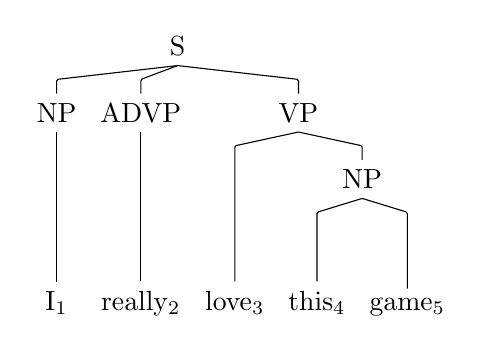
\begin{tikzpicture} [
				level distance=24pt,
				every tree node/.style={align=center,anchor=base},
				frontier/.style={distance from root=92pt},
				edge from parent/.style={draw,edge from parent path={(\tikzparentnode.south) {[rounded corners=0.5pt]-- ($(\tikzchildnode |- \tikzparentnode.south) + (0, -5pt)$) -- (\tikzchildnode)}}}
			]
			\Tree
			[.S
				[.NP I$_1$ ]
				[.ADVP really$_2$ ]
				[.VP love$_3$ [.NP this$_4$ game$_5$ ] ]
			];
		\end{tikzpicture}
		\caption{原始句法树}
		\label{fig:con-original-tree}
	\end{subfigure}
	\hfill
	\begin{subfigure}[b]{0.45\textwidth}
		\centering
		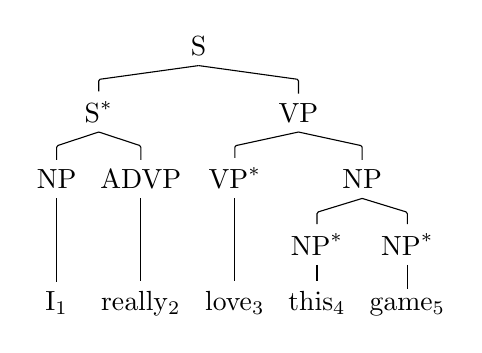
\begin{tikzpicture} [
				level distance=24pt,
				every tree node/.style={align=center,anchor=base},
				frontier/.style={distance from root=92pt},
				edge from parent/.style={draw,edge from parent path={(\tikzparentnode.south) {[rounded corners=0.5pt]-- ($(\tikzchildnode |- \tikzparentnode.south) + (0, -5pt)$) -- (\tikzchildnode)}}}
			]
			\Tree
			[.S
				[.$\textrm{S}^\ast$ [.NP I$_1$ ] [.ADVP really$_2$ ] ]
				[.VP
					[.$\textrm{VP}^\ast$ love$_3$ ]
					[.NP [.$\textrm{NP}^\ast$ this$_4$ ] [.$\textrm{NP}^\ast$ game$_5$ ] ]
				]
			];
		\end{tikzpicture}
		\caption{遵循乔姆斯基范式的左二叉化句法树}
		\label{fig:con-binaried-tree}
	\end{subfigure}
	\caption{
		成分句法树的例子.
		其中词性在这里被忽略
	}
	\label{fig:con-tree-full-figure}
\end{figure}

成分句法则旨在构建一个层次化的树结构。
如图\ref{fig:con-tree-full-figure},其中每个叶子结点是输入句子的每个词,而非终端结点作为区块(Constituents),如$\texttt{VP}_{3,5}$。
正式地,给定一个由$n$个词组成的句子$\boldsymbol{x}=w_1,\dots,w_{n}$,如图~\ref{fig:con-original-tree}所示,一棵成分句法树可以表示为$\boldsymbol{t}=\{((i, j),l)\mid 1\le i \le n,i \le j \le n,l \in \mathcal{L}\}$,其中$((i,j),l) \in \boldsymbol{t}$是一个包含$w_{i}...w_{j}$的区块,对应的句法标签为$l \in \mathcal{L}$。
本文中,为了方便模型处理,我们还将原始的树转换为了符合乔姆斯基范式(Chomsky Normal Form, CNF)的二叉树形式,如图~\ref{fig:con-binaried-tree}所示。
成分句法分析相比于依存句法而言,研究历史更加悠久,尽管目前没有依存句法技术那么流行,但是以其分析技术为基础衍生出了一系列在其他任务上的解析方法,例如UCCA语义分析 \citep{jiang-etal-2019-hlt}、嵌套命名实体识别 \citep{fu-etal-2021-nested}等等。

目前,针对句法分析任务,已经有大量的句法分析范式被提出,主要的有生成式方法、判别式方法,以及基于转移的方法、基于图的方法等等。
其中,基于图的方法尝试对每棵可能的句法树进行打分,然后选择一棵分值最高的树作为输出。
最简单的一阶方法将句法树分值分解为每个独立变量的分值之和,极大简化了模型建模。
与其他方法相比,基于图的方法无需设计复杂的转移系统,容易集成丰富的特征,可以达到很高的准确率,一直以来都是最流行的句法分析方法之一,因此也是本文所主要关注的句法分析方法。

传统的句法分析方法十分依赖于离散特征的人工设计和结构化建模。
由于缺乏对输入句子上下文的捕获能力,传统方法不得不手动设计诸如前缀、后缀、词性等特征,作为词输入的补充信息。
此外,显式的的树约束也是不可或缺的,模型依赖于Max Margin或TreeCRF等训练方法来全局最大化一棵树的分值/概率。

最近,由于深度神经网络的强大上下文编码能力,句法分析器的方法愈来愈有简单化的趋势。
作为依存句法和成分句法领域各自最有代表性的模型,\citet{dozat-etal-2017-biaffine}的依存句法分析器Biaffine Parser 和\citet{stern-etal-2017-minimal}的成分句法分析器正是符合这样的潮流。
其中Biaffine Parser: 1)采用了一个诸如双向LSTM或Transformer \citep{vaswani-2017-attention}这样强大的编码器;2)采取了简单的头选择训练损失函数。
类似地,\citet{stern-etal-2017-minimal}在双向LSTM编码器的基础上采取了Max Margin训练目标最大化正确树的分值,而\citet{gaddy-etal-2018-whats}更进一步,直接采取二分类方法判断短语树的每个组块是否存在。
这些方法由于建模简单,速度很快,因此一直是当前最为流行的句法分析方法。

有鉴于此,我们尝试在本文中将传统方法与现代的句法分析器做一个连接。
首先,我们在章节~\ref{cha:dep-crf}和章节~\ref{cha:con-crf}中采用了TreeCRF代替了当前流行的局部训练损失目标或者Max Margin方法。
与这些方法相比,TreeCRF的主要优势在于可以获得树/子树概率。
不同于没有上下界的分值,树/子树概率是评估解析置信度的更好指标,此外也可以作为一种软特征方便地作为下游任务的输入 \citep{zhang-etal-2019-syntax,zhang-etal-2020-syntax}。
主要限制TreeCRF应用的原因在于Inside-Outside算法的高复杂度问题,尤其是Outside过程,一般两倍慢于Inside。
对此,我们主要从两个方面尝试解决:
1)我们为Inside算法设计了精巧的批次化方法,使得TreeCRF能够利用GPU的并行计算能力大大加速;
2)得益于集成了自动求导机制的深度学习库的出现,我们无需和前人一样需要在CPU上进行完整的Inside-Outside过程得到梯度,而是将Outside过程由高效的反向传播机制代替。

此外,已经有很多工作证明,在模型中引入包含更多变量交互的高阶特征可以极大提升句法分析的准确率 \citep{mcdonald-pereira-2006-online,chen-manning-2014-fast,ji-etal-2019-graph}。
因此在章节~\ref{cha:dep-crf}和章节~\ref{cha:con-crf}中,我们在一阶模型的基础上引入了一个高阶TreeCRF的拓展。
为了能够对二阶子树特征打分,我们还参考Biaffine打分器为其设计了一个Triaffine机制。
结果表明,高阶TreeCRF在大多数数据集上都带来了显著的提升。

尽管可以应用批次化技术,高阶TreeCRF仍不可避免地加剧了推断算法效率低下的问题。
在机器学习社区中,研究者在针对推断算法高复杂度或者不可精确推断问题时,一个通常的做法是尝试采用近似推断算法。
因此在章节~\ref{cha:vi}中,我们还尝试了利用近似的平均场变分推断(Mean Field Variational Inference, MFVI)方法来代替高阶TreeCRF。
和其他同样在句法分析中广泛应用的近似推断算法,例如循环置信传播 \citep{smith-eisner-2008-dependency}和对偶分解 \citep{martins-etal-2009-concise},相比,MFVI的效率更高,收敛更快,并且通常可以达到更好的结果 \citep{wang-etal-2019-second}。
此外,MFVI能够方便的得到树/子树的概率,这保留了TreeCRF的优势。
我们在依存句法和成分句法分析两种范式中分别设计了两种不同的因子图以及变分推断迭代算法,结构表明MFVI在达到和高阶TreeCRF相接近的性能的同时,显著提升了句法模型的解析速度。

\section{数据集和评价指标}

\begin{table}[tb!]
    \centering
    \caption{依存句法分析数据集的数据统计,包含句子数和标签数.}
    \begin{tabular}{lrrr|c}
        \toprule
                & \#Train & \#Dev & \#Test & \#labels \\[1pt]
        \midrule
        % \\[-8pt]
        PTB     & 39,832  & 1,700 & 2,416  & 45       \\
        CoNLL09 & 22,071  & 1,762 & 2,556  & 41       \\
        NLPCC19 & 29,991  & 4,098 & 8,295  & 22       \\
        \bottomrule
    \end{tabular}
    \label{table:dep-statistics}
\end{table}

\noindent\textbf{数据.}
对于依存句法分析,我们在13个语言的27个数据集上进行了实验和分析,包含两个广泛使用的数据集:英语的斯坦福依存规范 \citep{chen-manning-2014-fast}的宾州树库(Penn Treebank, PTB)和中文的CoNLL09数据 \citep{hajic-etal-2009-conll}。
我们还采用了公开于NLPCC19跨领域句法分析任务的中文数据集 \citep{peng-etal-2019-overview},其中一共包含了四个源领域和三个目标领域。
方便起见,我们直接合并了四个领域的Train/Dev/Test数据到更大的数据集。
这些数据的一个特征是大部分句子都是利用基于主动学习的局部标注得到的。
表~\ref{table:dep-statistics}列出了相关数据的统计信息。
最后,遵循 \citet{ji-etal-2019-graph}和 \citet{zhang-etal-2019-empirical},我们在Universal Dependencies (UD) v2.2和v2.3上进行了实验。
我们采用了\citet{zeman-etal-2018-conll}使用的300维多语言预训练词向量,并采用CharLSTM表示作为输入。
对于UD2.2,为了和\citet{ji-etal-2019-graph}公平比较,我们和CoNLL18任务一样 \citep{zeman-etal-2018-conll},使用了毛文本,并且直接使用了他们的句子分割和符号化的结果。
对于UD2.3,为了与\citet{zhang-etal-2019-empirical}比较,我们报告的结果使用了正确词性。

对于成分句法分析,我们主要在三个中文和英文的数据集上进行实验。
前两个数据集,即PTB和CTB5.1,是句法分析社区中比较常用的两个数据集。
我们遵循了传统的Train/Dev/Test数据分割。
考虑到CTB5.1的Dev/Test都只有大约350句,为了得到更加稳定一致的结果,我们还在更大的CTB7数据上进行了实验,相关的数据分割设置参考了官方手册建议。
表~\ref{table:con-statistics}列出了相关数据的统计信息,其中UD的数据较多,因此不一一列举。
可以看到CNF转换引入了很多新的区块标签,其中大部分(大约75\%)都源于连续单链的折叠过程。

\begin{table}[tb!]
    \centering
    \caption{成分句法分析数据集的数据统计,包含句子数和标签数.
        对于``\#labels'',我们列出了原始树和CNF树对应的标签数.}
    \begin{tabular}{lrrr|cc}
        \toprule
               & \multirow{2}{*}{\#Train} & \multirow{2}{*}{\#Dev} & \multirow{2}{*}{\#Test} & \multicolumn{2}{c}{\#labels}       \\
               &                          &                        &                         & original                     & CNF \\[1pt]
        \midrule
        % \\[-8pt]
        PTB    & 39,832                   & 1,700                  & 2,416                   & 26                           & 138 \\
        CTB5.1 & 18,104                   & 352                    & 348                     & 26                           & 162 \\
        CTB7   & 46,572                   & 2,079                  & 2,796                   & 28                           & 265 \\
        \bottomrule
    \end{tabular}
    \label{table:con-statistics}
\end{table}

\noindent\textbf{评价指标.}
对于依存句法分析,我们使用无标签/有标签附着分值(Unlabeled/Labeled Attachment Score, UAS/LAS)作为主要的评价指标,其中UAS指头正确的词数占总词数之比,LAS则进一步还要求词的头正确的同时弧上的标签也正确。
评价时,PTB中的词性会被忽略掉。
对于局部标注的NLPCC19数据,我们采用了官方的评价脚本,直接忽略了没有正确头标注的词。
我们采用了Dan Bikel的随机解析评价比较器来进行显著性检验。

对于成分句法分析,在解析之后,我们将最佳的CNF树转化为\textit{n}-ary树再进行评价。
这里有必要提及一些有用的细节。
由于解码算法没有相应的约束,预测的最佳CNF树可能包含很多不合法的产生式。
以图~\ref{fig:con-binaried-tree}为例,模型可能输出$\texttt{VP}_{3,5} \rightarrow \texttt{PP}^{\ast}_{3,3} ~ \texttt{NP}_{4,5}$,其中 $\texttt{VP}$和$\texttt{PP}^{\ast}$是不兼容的。
在\textit{n}-ary后处理过程中,我们直接忽略了``$\mathtt{\ast}$''符号之前具体的字符串$\texttt{PP}$。
有鉴于此,如果解码的时候增加一定的约束,结果有可能进一步提高,这里我们留待作为后续的工作。
我们使用了标准的区块级别的准确率、召回率和$\mathrm{F}_1$值($\mathrm{P}$/$\mathrm{R}$/$\mathrm{F}_1$)作为评价指标,并使用\texttt{EVALB}工具\footnote{\url{https://nlp.cs.nyu.edu/evalb}}来评价。
特别地,一个例如$\texttt{VP}_{3,5}$的预测区块如果出现在了正确树中,那就被认为是正确的.\footnote{
	由于一些研究者可能会实现他们自己的评价脚本,为了比较的公平,需要澄清一些细节:
	1)一些诸如\texttt{\{-NONE-\}}的空区块在预处理的时候被移除了;
	2)评价的时候作为根结点的区块(英语里是\texttt{\{TOP,S1\}},中文里是空字符串) 被忽略了;
	3)包含一些例如\texttt{\{:,``,'',.,?,!\}}这些标点的区块也被忽略了;
	请注意中文标点会作为正常的字符被评价;
	4)一些在同一集合中的标签,例如\texttt{\{ADVP,PRT\}},被认为是等价的.}

\section{相关工作}
\label{sec:relworks}

\subsection{依存句法分析}

目前依存句法分析的两种主流方法分别是基于图的方法和基于转移的方法。
\textbf{基于图的方法}旨在从一个有向完全图中找到一棵概率(分值)最大的树,\textbf{基于转移的方法}将句法树的构建转化为一个移进和归约的动作序列,并寻求得到最优序列。

\citet{mcdonald-etal-2005-online}首先提出了基于图的训练方法。
他们提出采用基于动态规划的Eisner算法从有向完全图中得到分值最大的投影树,然后用Max Margin方法来训练。
后来\citet{mcdonald-etal-2005-non}将方法拓展到了非投影树解析领域,使用了ChuLiu/Edmods算法 \citep{chu-1965-shortest}得到分值最高的树。
由于学习和解码算法的复杂度很高,基于图的方法在给树打分时需要很强的独立性假设,其中最简单的弧分解假设认为树的每条弧相互独立(称为一阶模型),相应的树分值为所有弧的分值之和。
后来有研究者提出放宽独立性假设,将邻接兄弟、祖父、共同父亲等子结构的分值也引入树的打分中,基于此,他们提出了一系列的二阶 \citep{mcdonald-pereira-2006-online,carreras-2007-experiments}、三阶 \citep{koo-collins-2010-efficient}模型,并在依存句法上得到了可观的准确率提升。
解码时一阶方法通常采用Eisner和MST算法来进行投影/非投影解码,高阶方法在使用一阶算法解码时一般需要结合最小贝叶斯风险(Minimum Bayesian Risk, MBR )解码 \citep{smith-smith-2007-probabilistic}。
值得一提的是\citet{mcdonald-pereira-2006-online}发现二阶非投影解析是NP-hard问题,无法设计相应的动态规划结构融入高阶分值,因此基于图的高阶方法仅限于投影解析。

基于转移的方法则旨在将寻找句法树归约为搜索一个最优动作序列的问题。
一个转移系统一般由一个栈以及一个队列组成,分别储存部分解码的序列和未处理的词,接着系统定义了一系列的动作进行入栈/出栈、合并子树等操作,最终消耗完毕所有词,得到一棵完整句法树。
常见的转移系统有Arc-standard和Arc-eager等。
原始的基于转移的方法采用了局部的贪心算法来逐步预测每个动作,这可能导致错误传播(error propagation)的问题。
后来\citet{zhang-clark-2008-tale,huang-etal-2009-bilingually}引入了全局训练方法,并在解码时采用集束搜索(beam search),显著提升了准确率,达到和基于图方法相近的性能。

进入到深度学习时代,得益于神经网络编码器上下文编码能力的进步,有大量的工作尝试了不同的神经网络模型,
\citet{chen-manning-2014-fast}首先将前馈神经网络引入到基于转移的方法中,\citet{kiperwasser-goldberg-2016-simple,wang-chang-2016-graph}在基于图的模型中引入了双向LSTM编码器,\citet{li-etal-2019-attentive}则首次将Transformer用于依存句法分析模型,依存句法分析的性能得到了飞跃。
其中,\citet{dozat-etal-2017-biaffine}在3层双向LSTM编码器的基础上,采用了一个简单的基于头选择的训练目标,首次将PTB的LAS性能推进到了94.08。
这些模型大都采用了简单的一阶基于图的模型,而基于转移的方法渐渐式微,其中\citet{ma-etal-2018-stack}是最近的基于转移的工作之一,他们不再采用经典的转移系统,而是用Seq2Seq框架结合Pointer Network,达到了和基于图模型相近的性能。

近期开始有研究者探索将传统的结构化学习和高阶建模技术应用到在神经网络中。
\citet{zhang-etal-2019-empirical}探索了在一阶Biaffine Parser上结构化学习的作用。
他们在多语言数据上比较了局部头选择损失、全局Max Margin损失和TreeCRF损失的性能。
他们表明全局的TreeCRF损失总体上要稍微好于Max Margin损失,并且对大多数语言而言,结构化学习带来了虽然不多但是显著的LAS提升。
他们表明结构化学习,特别是TreeCRF,极大地提升了句子级匹配的准确率,这与我们的观察相仿。

\citet{falenska-kuhn-2019-non}则提出了一个在依存句法上的分析性工作。
通过将\citet{kiperwasser-goldberg-2016-simple}的一阶基于图的方法扩展到二阶,他们尝试探究有多少结构化上下文被双向LSTM编码器捕捉。
他们拼接3层LSTM的在$i,k,j$位置的输出向量来给邻接兄弟子树打分,并采用了Max Margin训练损失和二阶Eisner解码算法 \citep{mcdonald-pereira-2006-online}。
基于他们相对负面的结果和分析,他们认为高阶建模是多余的,因为双向LSTM已经可以有效的隐式捕捉足够的结构化上下文。
在我们的工作中,我们使用了一个更强的基线模型,并且得到了相比于他们的工作更显著的UAS/LAS提升。
特别地,我们进行了深入的分析,表明显式建模高阶信息可以帮助句法模型,因此与双向LSTM编码器是互补的。

\citet{ji-etal-2019-graph}引入了高阶结构信息,并在Biaffine Parser \citep{dozat-etal-2017-biaffine}上用图神经网络来隐式建模。
他们使用了多层的图注意力网络(Graph Attention Network,GAT) \citep{velickovic-etal-2018-graph}作为组块,每层GAT的每个节点通过集聚邻居节点信息产生新的表示。
通过多次迭代,一个节点渐渐的收集到多跳的高阶信息作为单条弧打分的全局证据。
训练时他们遵循了原始的头选择训练损失。
与此相对的,我们的工作采用的全局的TreeCRF损失并显式地将高阶分值引入到了Biaffine Parser。

\subsection{成分句法分析}

成分句法分析领域最简单的\textbf{生成式模型}为概率上下文无关文法(Probabilistic Context-Free Grammars, PCFGs)。
PCFGs将一棵句法树的概率分解为所有产生式$A\rightarrow B_1B_2\dots B_n$的概率之积,其中$A$代表非终端结点,$B$代表一个终端/非终端结点,并寻求最大化该概率。
\citet{collins-1997-three}在基于简单的头发现规则(head-finding rules)下为每个非终端结点$A$引入词汇化标记得到$A(w)$,将概率上下文无关文法拓展为了词汇化的概率上下文无关文法(Lexicalized PCFGs)。
这推动了生成式模型的广泛流行。
\citet{matsuzaki-etal-2005-probabilistic}和\citet{petrov-etal-2006-learning}(Berkeley Parser)利用隐变量对非终端结点进行自动标记,并通过EM算法来训练产生细粒度的上下文无关规则,该方法首次超越了Lexicalized PCFGs方法。
最近的工作中,\citet{dyer-etal-2016-recurrent}提出了循环神经网络文法(Recurrent Neural Network Grammars, RNNGs),在一个自顶向下的转移系统的基础上额外附加了一个生成动作$\textsc{Gen}(\cdot)$,最终模型建模句子和句法树的联合概率$p(\boldsymbol{x},\boldsymbol{y})$。
\citet{kuncoro-etal-2017-recurrent}对RNNGs进行了详细的消融性分析,发现转移系统中的栈结构最为重要,相应的他们的Stack-only RNNGs达到了当时成分句法分析的最佳性能。

与生成式模型相对的为\textbf{判别式模型},其中包含两种代表性方法,即基于转移的方法和基于图的方法。
和依存句法类似,基于转移的方法包含了一个栈以及一个缓存来存放已有句法树和未处理词,转移系统根据当前动作逐步处理词汇,并根据当前状态预测下一个动作,最终归约出一棵句法树。
根据树的迭代和子树归约的次序不同,存在三类转移系统,分别为基于后序(post-order)遍历(或自底向上)、基于前序(pre-order)遍历(或自顶向下)以及基于中序(in-order)遍历 \citep{liu-zhang-2017-order}的转移系统。
解码时通常都采用集束搜索。
基于转移的方法通常会遇到两个问题:1)曝光偏置(\emph{exposure bias}),即训练时模型通常面对的都是正确的动作,而解析时可能得到错误预测,根据错误动作继续进行预测时结果可能会越来越差;2)损失函数不匹配(\emph{loss mismatch}),转移系统的训练采用了局部动作级别损失而忽视了全局的结构指标。
对于第一个问题,通常的解决办法为动态指导(dynamic oracle),即在预测偏离正确树之后指导模型向着错误相对更少的状态转移,例如在标签预测时,将不存在于正确树的区块的标签的答案设计为$\emptyset$,\citet{cross-huang-2016-span}应用了动态指导并给出了详细证明。
对于第二个问题,\citet{fried-klein-2018-policy}采取了策略梯度(policy gradient)的方法解决,策略梯度定义了一个风险函数(通常为负$\mathrm{F}_1$值),训练时模型用期望风险最小化的训练目标代替了局部动作损失。

我们的成分句法分析器基于判别式的高性能基于双向LSTM编码器的现代神经网络分析器 \citep{stern-etal-2017-minimal},在基于图的模型上利用了minus feature \citep{cross-huang-2016-span}进行区块的打分。
最近有很多工作都参考了\citet{stern-etal-2017-minimal}。
\citet{gaddy-etal-2018-whats}尝试分析什么样的,以及有多少上下文被双向LSTM隐式编码。
\citet{kitaev-klein-2018-constituency}将2层双向LSTM替换为自注意力层,并通过分离上下文和位置注意力,发现了可观的提升。
与此对应的,我们的工作表明通过合理的设置双向LSTM,例如Dropout策略,\citet{stern-etal-2017-minimal}的分析器可以超过\citet{kitaev-klein-2018-constituency}的结果。
请注意\citet{kitaev-klein-2018-constituency}的工作中使用了很大的词向量。

与此同时,近期有许多工作没有显式考虑结构化约束或者CKY解码,极大简化了成分句法分析任务。
\citet{gomez-rodriguez-vilares-2018-constituent}通过对每个词设计复杂的标签编码树信息,尝试采用序列标注方法解决成分句法分析任务。
\citet{vilares-etal-2019-better}通过一系列的增强技术,例如多任务学习和策略梯度,进一步增强了序列标注方法。
\citet{shen-etal-2018-straight}提出对于正确树中的每个邻居词对预测一个数值距离,并应用自底向上的贪婪解码找到一棵最优的树。
然而,所有上面的工作仍然在解析性能上极大的落后于主流的方法。

\subsection{TreeCRF加速方法}

TreeCRF方法在计算句法树概率时需要在全局空间上对句法树的分值进行归一化,这带来了效率低下的问题,因此目前关于TreeCRF的句法分析的工作相对较少。
\citet{finkel-etal-2008-efficient}首先提出了一个基于非神经网络的引入丰富特征的TreeCRF成分句法分析器。
\citet{durrett-klein-2015-neural}拓展了\citet{finkel-etal-2008-efficient}的工作,使用一个带非线性激活的前馈神经网络来打分产生式。
这两个工作都在CPU上显式进行了Inside-Outside计算,带来了严重的效率问题。

与此对应的,和TreeCRF类似进行结构化学习,但是无需全局归一化的Max Margin方法相对要更加流行。
\citet{taskar-etal-2004-max}首次在依存句法上提出Max Margin解析,训练时最大化正确句法树和其他可能句法树的分值间隔,后来\citet{mcdonald-etal-2005-online,mcdonald-etal-2005-online}都采用了这种学习目标,而近期的代表性工作中,\citet{wang-chang-2016-graph,kiperwasser-goldberg-2016-simple}均采用了Max Margin训练。
当前流行的成分句法模型 \citep{stern-etal-2017-minimal,kitaev-klein-2018-constituency,zhou-zhao-2019-head}通常也采用了Max Margin训练方法。

最近也有工作提出对TreeCRF等结构化学习算法进行加速。
\citet{zhang-etal-2017-dependency-parsing,jiang-etal-2018-supervised,li-etal-2019-semi-supervised}作为最近的基于TreeCRF的工作,采用了Cython Programming并结合多线程,在CPU上加快了Inside-Outside的计算。
类似地,\citet{kitaev-klein-2018-constituency}将Cython Programming应用到了Max Margin训练上。
而在本文中,我们从两个方面来加速TreeCRF算法:1)批次化技术;2)用基于自动求导的反向传播代替Outside算法。

对于序列标注任务而言,批次化很直接,并且已经被很好的解决,比如NCRF++的实现\footnote{\url{https://github.com/jiesutd/NCRFpp}},但是在树形结构中这个要复杂得多。
我们首次提出分别在依存和成分句法上批次化树形结构的Inside和Viterbi(Eisner/CKY)计算,以便于利用GPU加速。

\citet{eisner-2016-inside}在成分句法分析上提出了一个关于Outside算法和反向传播机制等价性的理论证明,并同样讨论了其他类似于依存文法的范式。
我们在本文的工作中借鉴了他们的理论性工作,在依存和成分文法中用反向传播完全取代了Outside算法,显著提升了解析效率。
作为一个经验性分析,我们相信我们的尝试能够让TreeCRF在现实系统中应用起来。

Torch-Struct\footnote{\url{https://github.com/harvardnlp/pytorch-struct}} \citep{rush-2020-torch}是我们的方法之外一个同期独立完成的工作,他们同样为依存句法和成分句法实现了批次化的Eisner/CKY算法,并且和我们一样,将Outside算法用Inside过程以及基于自动求导的反向传播代替。
然而,Torch-Struct旨在实现通用目的的结构化预测算法。
与此不同的是,我们着力于复杂的解析器模型,并力求达到依存句法分析和成分句法分析在准确率和效率上的最佳性能。
此外,Torch-Struct关注于一阶算法,而我们分别还在两种句法分析范式中引入了二阶的Eisner/CKY算法,并做了大量的针对性实验和分析。

\subsection{近似推断方法}
针对句法分析的推断算法,我们关注于两个问题:1)最大后验概率推断(Maximun \textit{a posteriori} inference, MAP inference),即得到后验概率最大化的句法树;2)边缘概率推断(Marginal inference),即得到句法树中每个变量的边缘概率。
尽管为推断算法引入高阶特征,能够帮助模型准确率的提升 \citep{mcdonald-pereira-2006-online,carreras-2007-experiments,koo-collins-2010-efficient,ma-zhao-2012-fourth},
然而这种通常导致两种情况:1)相应的精确推断算法有很高的复杂度;2)无法得到一个可精确推断的动态规划算法来计算目标结构的概率。
对于前者,我们可以考虑批次化方法和自动求导等技术,利用GPU并行计算的能力,降低算法复杂度。
而对于后一种情况,通常我们不得不考虑近似方法。
由于不可精确推断问题的广泛存在,因此一直以来近似推断算法在NLP社区都有很多都应用。

\citet{martins-etal-2009-concise}将依存句法分析问题近似为整数线性规划(Integer Linear Programming, ILP)问题。
与传统算法相比,他们利用了大量的局部和全局的丰富特征,例如兄弟、祖父特征和价键特征,作为线性约束,用ILP来求解,保证输出是一棵合法的依存树。
\citet{koo-etal-2010-dual}将非投影依存句法分析形式化为对偶分解(Dual Decomposition, DD)问题,将一个难以求解的问题分解为若干个可求解的子问题,例如可以将输出树的问题分解到单条弧、邻接兄弟、双头等子结构上 \citep{martins-etal-2011-dual}。

另一个和本文采用的平均场变分推断高度相关的方法是循环置信传播(Loopy Belief Propagation, LBP)。
LBP定义了一个包含多种局部和全局特征的由变量和因子构成的因子图,接着算法迭代式地让因子(变量)收集邻居变量(因子)的信息,最终收敛后得到后验概率。
\citet{smith-eisner-2008-dependency,gormley-etal-2015-approximation}在依存句法分析上引入了LBP。
除了上面提到的兄弟(\textsc{Sib})、祖父(\textsc{Grand})因子,他们还引入了丰富的全局因子,例如\textsc{Exactly1}约束每个词有且仅有一个头,\textsc{Tree}要求所有词必须组成一棵树等等。
\citet{naradowsky-etal-2012-grammarless}将LBP引入到了成分句法分析,也采用了类似的高阶因子(如\textsc{Tree})在成分句法上的变体。
与精确算法相比,LBP可以用可接受的复杂度引入大量全局因子,并为模型带来了可观的性能收益。

还有一些工作同时使用了上述的近似算法。
\citet{auli-lopez-2011-comparison}在组合范畴文法中同时采用了LBP \citep{smith-eisner-2008-dependency}以及DD \citep{koo-etal-2010-dual},取得了最佳性能,并对两种方法做了经验性比较。
\citet{martins-etal-2010-turbo}提出了在非投影依存句法分析中同时利用了LBP \citep{smith-eisner-2008-dependency}以及ILP \citep{martins-etal-2009-concise}方法,表明两种方法采用了一致的因子图,并在局部近似的目标函数的理念上是相一致的。

近期在神经网络模型上,涌现出了大量的关于近似推断在语义角色标注 \citep{li-etal-2020-high}、序列标注 \citep{wang-etal-2020-ain}等结构化预测任务等上的应用。
\citet{wang-etal-2019-second}首次在基于图的语义依存分析上提出了二阶模型,并采用LBP和MFVI作为近似算法,观察到了两种推断算法相似的性能提升。
\citet{wang-tu-2020-second}首次在依存句法分析中引入了MFVI,他们采用了兄弟、组合和共同父亲这三种二阶特征。
我们的依存模型中采用的基于头选择的MFVI参考了\citet{wang-tu-2020-second}的更新方法,但是为了和精确推断算法公平比较,本文中我们只保留了兄弟特征。
上述工作引入了近似推断算法之后都达到了和精确推断可比较的结果,同时速度上大大提升,这和我们的发现是一致的。

\section{章节和内容安排}

本文共分为五个章节,各章节具体安排如下:

第一章:绪论.
本章介绍本文中每个工作的任务背景和意义,并阐述一下与工作相关的有关文献的进展和内容,以及与我们方法的对比。

第二章:基于树形条件随机场的高阶依存句法分析方法.
本章在当前最佳的依存句法分析器的基础上,提出了一个二阶树形条件随机场的拓展,进一步提升了句法分析的性能。
为了解决效率问题,我们还提出了批次化技术在GPU上对训练和解码算法进行加速,以及用高效的反向传播代替Outside算法。

第三章:基于树形条件随机场的高阶成分句法分析方法.
本章将树形条件随机场的应用到了神经成分句法分析器当中。
我们应用了和依存模型一样的加速方法解决了树形条件随机场效率低下的问题。
我们提出了一个简单的两阶段解析方法,来进一步提升分析器的效率。
参考依存句法的模型架构和参数设置,我们还为解析器引入了新的打分方法,以及有效的Dropout策略,使得解析器达到了新的最佳水平。

第四章:基于变分推断的高效句法分析方法.
本章在前面章节提出的高阶句法分析器的基础上,提出利用平均场变分推断方法来近似推断后验概率。
与精确推断的高阶TreeCRF方法相比,变分推断显著降低了复杂度,并达到了和高阶TreeCRF接近或相当的结果。

第五章 总结与展望.
本章总结本文的主要内容,并展望后续可能的句法分析方法。

\chapter{基于树形条件随机场的快速精准成分句法分析}
\label{cha:con-crf}

本章节提出了一个基于树状条件随机场的快速精准的神经成分句法分析器.
估计概率分布一直是自然语言处理领域的一个核心问题.
但是,在深度学习时代和前深度学习时代,不同于线性链条件随机场(linear chain CRF)在序列标注任务中的大量应用,由于Inside-Outside算法的高复杂度,还很少有工作将树形条件随机场应用到成分句法分析任务当中.
这里我们提出应用树状条件随机场到成分句法分析,核心的想法是批次化计算损失函数用到的Inside算法,使其能够支持在GPU上的大规模张量并行计算,与此同时结合基于高效自动求导机制的反向传播,避免了复杂的Outside算法的计算.
我们同样提出一个简单的两阶段解析方法,bracketing-then-labeling,来进一步提升分析器的效率.
为了提升解析的性能,受依存句法分析器的启发,我们引入了一个基于边界表示和仿射注意力的新打分架构,以及一个有效的Dropout策略.
在PTB、CTB5.1和CTB7上的实验表明我们的两阶段条件随机场分析器在使用和不使用BERT的两种设置上,达到了新的最佳性能,并且解析速度达到了1,000句每秒.

\section{引言}\label{sec:con-intro}

\begin{figure}[tb!]
	\centering
	\begin{subfigure}[b]{0.45\textwidth}
		\centering
		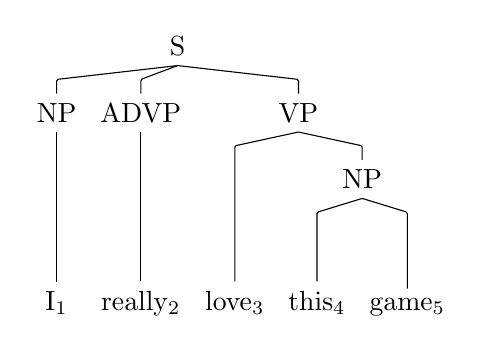
\begin{tikzpicture} [
				level distance=24pt,
				every tree node/.style={align=center,anchor=base},
				frontier/.style={distance from root=92pt},
				edge from parent/.style={draw,edge from parent path={(\tikzparentnode.south) {[rounded corners=0.5pt]-- ($(\tikzchildnode |- \tikzparentnode.south) + (0, -5pt)$) -- (\tikzchildnode)}}}
			]
			\Tree
			[.S
				[.NP I$_1$ ]
				[.ADVP really$_2$ ]
				[.VP love$_3$ [.NP this$_4$ game$_5$ ] ]
			];
		\end{tikzpicture}
		\caption{原始句法树}
		\label{fig:con-original-tree}
	\end{subfigure}
	\hfill
	\begin{subfigure}[b]{0.45\textwidth}
		\centering
		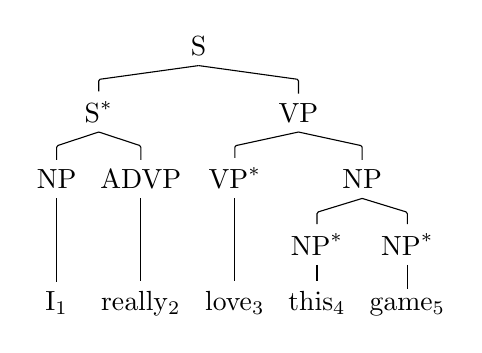
\begin{tikzpicture} [
				level distance=24pt,
				every tree node/.style={align=center,anchor=base},
				frontier/.style={distance from root=92pt},
				edge from parent/.style={draw,edge from parent path={(\tikzparentnode.south) {[rounded corners=0.5pt]-- ($(\tikzchildnode |- \tikzparentnode.south) + (0, -5pt)$) -- (\tikzchildnode)}}}
			]
			\Tree
			[.S
				[.$\textrm{S}^\ast$ [.NP I$_1$ ] [.ADVP really$_2$ ] ]
				[.VP
					[.$\textrm{VP}^\ast$ love$_3$ ]
					[.NP [.$\textrm{NP}^\ast$ this$_4$ ] [.$\textrm{NP}^\ast$ game$_5$ ] ]
				]
			];
		\end{tikzpicture}
		\caption{遵循乔姆斯基范式的左二叉化句法树}
		\label{fig:con-binaried-tree}
	\end{subfigure}
	\caption{
		成分句法树的例子.
		其中词性在这里被忽略
	}
	\label{fig:con-tree-full-figure}
\end{figure}

给定一个句子,成分句法分析旨在构建一个层次化的树结构. 如图\ref{fig:con-tree-full-figure},其中每个叶子结点是输入句子的每个词,而非终端结点作为区块(Constituents),如\texttt{$VP_{3,5}$}.

成分句法分析是自然语言处理领域一个基础但是富有挑战性的任务.
由于诸如宾州树库(Penn Treebank,PTB)、中文宾州树库(Penn Chinese Treebank,CTB)等大规模树库的标注,成分句法分析吸引了一大批研究者的关注.
同样的,句法分析输出的句法树也被证明对于大量的下游任务\cite{akoury-etal-2019-syntactically,wang-etal-2018-tree}都有用.

作为最有影响力的工作之一,\cite{collins-1997-three}概率上下文无关文法 (Probabilistic Context-Free Grammars,PCFGs)扩展到了词汇化文法(Lexicalized PCFGs).
由此开始,成分句法分析方法一直是这样的生成式模型(generative models)占据主导地位,并且其中广泛使用的Berkeley Parser采用了带隐式非终端结点标注的非词汇化概率上下文无关文法(Unlexicalized PCFGs)\cite{matsuzaki-etal-2005-probabilistic,petrov-klein-2007-improved}.
而在判别式方法(discriminative models),存在着两种主要方向.
第一种采取了以动态规划解码为基础的基于图的方法,训练时使用局部max-entropy估计\cite{kaplan-etal-2004-speed}或者全局max-margin方法\cite{taskar-etal-2004-max}.
第二类则通过基于贪婪解码或者集束搜索(beam search)产生shift-reduce这样的转移序列来构建一棵树,这种方法被称为基于转移的方法\cite{sagae-lavie-2005-classifier,zhu-etal-2013-fast}.

最近,得益于深度神经网络在上下文表示方面令人印象深刻的发展,成分句法分析取得了显著的进展.
其中,\cite{cross-huang-2016-span}的基于转移的分析器,以及\cite{stern-etal-2017-minimal}的基于图的分析器是两个具有代表性的工作.
作为判别式模型,两个分析器有很多的共同点,他们都使用了1)多层双向LSTM作为编码器;2)从双向LSTM的输出得到的minus features作为区块的表示;3)利用MLP层来为区块打分;4)max-margin的训练损失函数.
后续的大多数工作\cite{gaddy-etal-2018-whats,kitaev-klein-2018-constituency}的主要设置都和这两个分析器一样, 并且都相比传统的非神经网络模型达到了更好的准确率,这特别是得益于由在大规模无标记文本上训练的语言模型输出的上下文词表示的使用\cite{peters-etal-2018-deep,devlin-etal-2019-bert}.

然而尽管有这些显著的进展,现有的成分句法分析的研究仍然受两个相互关联的缺点困扰.
首先,解析速度(训练速度同理)很慢,并且很难满足现实系统的需要.
其次,显式的树/子树概率建模的缺失一定程度上影响来分析器输出的利用.
一方面,估计概率分布一直是自然语言处理领域的核心问题\cite{le-zuidema-2014-inside}.
另一方面,与没有上下姐的树的分值相比,树的概率可以作为一种软特征,更好的被更高层级的任务所利用\cite{jin-etal-2020-relation},且子树的边缘概率可以支持更加复杂的最小贝叶斯风险解码\cite{smith-smith-2007-probabilistic}.

事实上,\cite{finkel-etal-2008-efficient,durrett-klein-2015-neural}都通过建模树的条件概率$p(\boldsymbol{t}\mid\boldsymbol{x})$,提出了基于CRF\cite{lafferty-etal-2001-crf}的成分句法分析器.
但是,由于损失函数和梯度计算需要的Inside-Outside算法的高复杂度(尤其是Outside算法),这些模型都极端低效.
而在深度学习时代,由于以前所有的工作都直接在CPU上运行Inside-Outside算法,而让模型频繁在CPU和GPU切换所需要的时间代价是昂贵的,因此效率问题变得更加严重.

本章节通过极大拓展\cite{stern-etal-2017-minimal}的基于图的分析器,提出了一个CRF成分句法分析器.
主要的贡献在于我们为损失函数和梯度能够在GPU上能够直接计算,类似于章节\ref{cha:dep-crf},我们提出了Inside算法的批次化方法.
与此同时,我们发现Outside算法的可以通过自动的反向传播机制被高效的完成,这验证了\cite{eisner-2016-inside}出色的理论性能做,使得outside过程与Inside一样高效.
类似的,我们也批次化了CKY(Cocke–Kasami–Younger)算法,以支持高效的解码.

总体而言,我们做了如下的贡献.
\begin{itemize}
    \item 为了直接建模树和子树的概率,我们首次提出了一个快速精准的CRF成分句法分析器.
          通过批次化技术支持Inside算法和CKY算法在GPU上的直接计算,长期以来一直困扰句法分析社区的效率问题在这里被很好的解决了.

    \item 我们提出了一个两阶段的解析方法bracketing-then-labeling:先产生无标记树骨干树(bracketing)再标注标签(labeling)的解析方法,这不仅更加高效,并且达到了比一阶段解析方法稍好的性能.

    \item 我们提出了基于区块表示的一个新的打分架构,以及基于仿射注意力机制的打分方法,比minus-feature方法表现的更好.
          我们同样表明,通过更好的模型及参数设置,比如Dropout,解析的性能可以被极大提升.

    \item 在中英文的三个基准数据集上的实验表明,我们提出的两阶段解析方法在使用BERT和不使用BERT\cite{devlin-etal-2019-bert})的两种设置下,性能上达到了新的最佳水准.
          解析速度方面,我们的分析器可以达到1,000句每秒的解析速度.
\end{itemize}

\begin{figure}[tb]
    \centering
    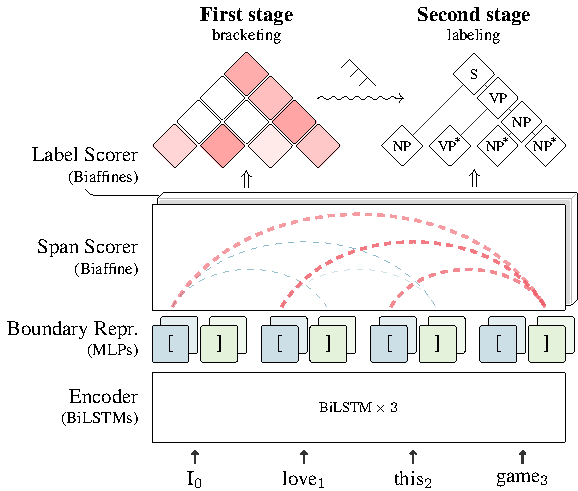
\includegraphics [scale=1.2]{figures/con-framework.pdf}
    \caption{模型架构.}
    \label{fig:con-framework}
\end{figure}

\section{两阶段CRF解析}\label{sec:2stage-parsing}

正式地,给定一个由$n$个词组成的句子$\boldsymbol{x}=w_0,\dots,w_{n-1}$,如图~\ref{fig:con-tree-original}所示,一棵成分句法树可以表示为$\boldsymbol{t}$,其中$(i,j,l) \in \boldsymbol{t}$是一个包含$w_{i}...w_{j}$的区块,对应的句法标签为$l \in \mathcal{L}$.
一棵树同样可以被分解为两个部分,即,$\boldsymbol{t}=(\boldsymbol{y}, \boldsymbol{l})$,其中$\boldsymbol{y}$是一棵无标签树(又称为bracketed tree),而$\boldsymbol{l}$是树中所有区块的标签按一定顺序产生的标签序列.
区块$(3,5,\texttt{VP})$可以等价表示为$\texttt{VP}_{3,5}$.

为了能够适应Inside算法和CKY算法,我们用NLTK工具包\footnote{\url{https://www.nltk.org}}将原始的树转换为了遵循乔姆斯基范式(Chomsky Normal Form,CNF)的二叉树形式,如图~\ref{fig:con-binaried-tree}所示.
特别地,连续的单链产生式被压缩为了一个标签,比如$\texttt{X}_{i,j} \rightarrow \texttt{Y}_{i,j}$会被压缩为一个$\texttt{X+Y}_{i,j}$.
根据前置实验,我们在二叉化原始树的时候,采用了左二叉.
在用CKY解码获得一棵最佳的树之后,CNF树会被恢复为原来的\textit{n}-ary形式.

\subsection{模型定义}\label{sub@sec:model-definition}

在这份工作中,我们对成分句法分析采用了一个两阶段的解析框架bracketing-then-labeling.
这与传统的一阶段解析方法\cite{stern-etal-2017-minimal,gaddy-etal-2018-whats}相比,不仅简化了模型架构,同样也提升了效率.

\noindent\textbf{第一阶段:bracketing.}
给定句子$\boldsymbol{x}$,第一阶段的目标是找到一个最优的无标签树$\boldsymbol{y}$.
一棵树的分值被分解为所有包含的区块的分值.
\begin{equation} \label{eq:tree-score}
    \mathrm{s}(\boldsymbol{x},\boldsymbol{y}) = \sum\limits_{(i,j)\in \boldsymbol{y}}\mathrm{s}(i,j)
\end{equation}
对于CRF,条件概率为
\begin{equation}\label{eq:tree-prob}
    \begin{split}
        & p(\boldsymbol{y}\mid\boldsymbol{x})  = \frac{\exp({\mathrm{s}(\boldsymbol{x},\boldsymbol{y}))}}{Z(\boldsymbol{x}) \equiv \sum\limits_{\boldsymbol{y'} \in \mathcal{Y}(\boldsymbol{x})} {\exp({\mathrm{s}(\boldsymbol{x},\boldsymbol{y'}))}}}
    \end{split}
\end{equation}
其中$Z(\boldsymbol{x})$被称为partition term,$\mathcal{Y}(\boldsymbol{x})$是输入句子$\boldsymbol{x}$对应的所有合法句法树的集合.

给定所有的区块分值$\mathrm{s}(i,j)$,我们可以用CKY算法来找到一棵最优的无标签句法树$\hat{\boldsymbol{y}}$.
\begin{equation} \label{eq:tree-argmax}
    \hat{\boldsymbol{y}} = \arg\max_{\boldsymbol{y}} \mathrm{s}(\boldsymbol{x}, \boldsymbol{y}) = \arg\max_{\boldsymbol{y}} p(\boldsymbol{y} \mid \boldsymbol{x})
\end{equation}

\noindent\textbf{第二阶段:labeling.}
给定一个句子$\boldsymbol{x}$和一棵树$\boldsymbol{y}$,第二阶段独立地给每个区块$(i,j) \in \boldsymbol{y}$预测一个标签.
\begin{equation} \label{eq:label-argmax}
    \hat{l} = \arg\max_{l \in \mathcal{L}} \mathrm{s}(i,j,l)
\end{equation}
请注意训练时我们使用正确的无标签树来进行损失函数的计算.
对于一个长度为$n$的句子,所有的CNF树都包含同样$2n-1$多个的区块.
因此,这一阶段的时间复杂度为$O(n|\mathcal{L}|)$.

\noindent\textbf{时间复杂度分析.}
CKY的时间复杂度为$O(n^3)$.
因此,我们两阶段解析方法的总时间复杂度为$O(n^3+n|\mathcal{L}|)$.
相对应的,对于一阶段解析的CKY而言,算法需要为所有$n^2$个区块决定最优的标签,因此需要$O(n^3+n^2|\mathcal{L}|)$,其中$|\mathcal{L}|$通常来说都很大(比如对于表~\ref{table:con-statistics}中的英语来说为138).

\subsection{打分架构}

本章节引入了给区块和标签打分的模型架构,如图~\ref{fig:con-framework},大部分设置都遵循\cite{stern-etal-2017-minimal},除了两个重要的修改:1)针对分值计算的边界表示和仿射注意力;2)和\cite{Timothy-d17-biaffine}一样的更好的参数设置.

\noindent\textbf{模型输入.}
对于第$i$个词,其对应的输入向量$\mathbf{e}_i$是词向量和字级别表示的拼接:
\begin{equation} \label{eq:token-representation}
    \mathbf{e}_i = \mathbf{e}^{word}_i \oplus \mathrm{CharLSTM}(w_i)
\end{equation}
其中$\mathrm{CharLSTM}(w_i)$是将字序列输入到双向LSTM一样的输出向量\cite{lample-etal-2016-neural}.
以前的工作表明将词性表示用$\mathrm{CharLSTM}(w_i)$代替会带来稳定的提升\cite{kitaev-klein-2018-constituency}.
这同样简化了模型,因为不再需要额外预测词性.

\noindent\textbf{双向LSTM编码器.}
我们在输入向量上应用了三层双向LSTM以得到上下文表示.
我们分别用$\mathbf{f}_i$和$\mathbf{b}_i$来表示词$w_i$在顶层LSTM的前向和后向输出向量.

在这里,我们借用了大部分\cite{Timothy-d17-biaffine}的依存句法分析器的参数设置(参考章节\ref{sec:dep-exps}).
我们发现其中的Dropout设置对于解析性能特别关键,这和原始的实现\cite{stern-etal-2017-minimal}有两方面的不同.

首先,对于每个词$w_i$,$\mathbf{e}^{word}_i$和$\mathrm{CharLSTM}(w_i)$都作为一个整体被dropout,要么保持版本,要么称为$\mathbf{0}$向量.
如果其中一个向量被设置为了$\mathbf{0}$,则另一个会被乘以2倍作为补偿.
其次,相同LSTM层在不同的时间步(词)共享相同的dropout掩码\cite{yarin-etal-2016-dropout}.

\noindent\textbf{边界表示.}
对于每个词$w_i$,我们参考\cite{stern-etal-2017-minimal}的做法来组成上下文词向量\footnote{我们的前置实验表明$\mathbf{f}_i \oplus \mathbf{b}_{i+1}$相比于$\mathbf{f}_i \oplus \mathbf{b}_i$有稳定的提升. 可能的原因是$\mathbf{f}_i$和$\mathbf{b}_i$都使用$\mathbf{e}_i$作为输入,因此提供的信息冗余.}
\begin{equation}
    \mathbf{h}_i = \mathbf{f}_i \oplus \mathbf{b}_{i+1}
\end{equation}
$\mathbf{h}_i$的维度为800.

不同于直接应用一个单一的MLP层到$\mathbf{h}_i$上,我们发现一个词在一棵给定树的所有的区块中都必须作为其左边界或右边界.
因此,我们应用来两个MLP层来做这样的区分,并且分别获取左边界和右边界的表示向量.
\begin{equation}
    \label{mlp-borlders}
    \mathbf{r}_i^{l}; \mathbf{r}_i^{r} =\mathrm{MLP}^{l} \left( \mathbf{h}_i \right); \mathrm{MLP}^{r} \left( \mathbf{h}_i \right)
\end{equation}
$\mathbf{r}_i^{l/r}$的维度$d$为500.
正如\cite{Timothy-d17-biaffine}所指出的,MLP层缩减了$\mathbf{h}_i$的维度,并且更重要的是只保留了句法相关的信息,因此能够减轻过拟合的风险.

\noindent\textbf{仿射打分.}
给定边界表示,对于候选区块$(i,j)$,我们在左边界词$w_i$的表示和右边界词$w_j$的表示上利用仿射注意力为该区块打分.
\begin{equation} \label{eq:biaffine}
    \mathrm{s}(i,j) =  \left[
        \begin{array}{c}
            \mathbf{r}_{i}^{l} \\
            1
        \end{array}
        \right]^\mathrm{T}
    \mathbf{W} \mathbf{r}_{j}^{r}
\end{equation}
其中$\mathbf{W} \in \mathbb{R}^{d \times d}$.

计算区块标签的分值$\mathrm{s}(i,j,l)$使用的是类似的方式.
需要在$\mathbf{h}_i$上应用额外两层MLP来获取相应的边界表示$\bar{\mathbf{r}}^{l/r}_i$(维度为$\bar{d}$).
接着我们使用$|\mathcal{L}|$个Biaffine($\mathbb{R}^{\bar{d} \times \bar{d}}$)来获取所有标签的分值.
由于$|\mathcal{L}|$非常大,我们对于$\bar{\mathbf{r}}^{l/r}_i$使用了稍小的维度$\bar{d}=100$(对于${\mathbf{r}}^{l/r}_i$则是500)以减轻内存和计算负担.

\noindent\textbf{前人打分方法.}
\cite{stern-etal-2017-minimal}对双向LSTM的输出使用了minus featured方法来得到区块的表示\cite{wang-chang-2016-graph,cross-huang-2016-span},然后用MLP层得到区块的分值.
\begin{equation} \label{eq:minus-score}
    \mathrm{s}(i,j)=\mathrm{MLP}(\mathbf{h}_{i}-\mathbf{h}_{j})
\end{equation}
在实验部分我们表明我们的打分方法要明显更优越.

\subsection{训练损失函数}

对于一个训练的例子$(\boldsymbol{x},\boldsymbol{y},\boldsymbol{l})$,训练损失函数由两部分组成.
\begin{equation} \label{eq:final-loss}
    \mathit{L(\boldsymbol{x}, \boldsymbol{y}, \boldsymbol{l})} = \mathit{L}^{bracket}(\boldsymbol{x}, \boldsymbol{y}) + \mathit{L}^{label}(\boldsymbol{x}, \boldsymbol{y}, \boldsymbol{l})
\end{equation}
第一项是句子级的全局CRF损失,目的是最大化树的条件概率:
\begin{equation}\label{eq:bracket-loss}
    \begin{split}
        \mathit{L}^{bracket}(\boldsymbol{x},\boldsymbol{y})
        &= -\mathrm{s}(\boldsymbol{x}, \boldsymbol{y}) + \log Z(\boldsymbol{x})
    \end{split}
\end{equation}
其中$\log Z(\boldsymbol{x})$可以利用Inside算法在$O(n^3)$的时间复杂度内被计算.

第二项是在labeling阶段,区块级别的标准交叉熵损失函数.

\section{高效的训练和解码}
\label{sec:efficient-training-decoding}

\begin{algorithm}[tb]
  \caption{批次化的Inside算法.}
  \begin{algorithmic}[1]
    \setlength{\commentindent}{.3\textwidth}
    \setlength{\algorithmicindent}{1.5em}
    \renewcommand{\algorithmiccomment}[1]{\unskip\hfill\makebox[\commentindent][l]{$\rhd$~#1}\par}
    \LetLtxMacro{\oldalgorithmic}{\algorithmic}
    \renewcommand{\algorithmic}[1][0]{%
      \oldalgorithmic[#1]%
      \renewcommand{\ALC@com}[1]{%
        \ifnum\pdfstrcmp{##1}{default}=0\else\algorithmiccomment{##1}\fi}%
    }
    %\begin{spacing}{1.2}
    % \begin{footnotesize}
    % \STATE $\forall 0 \le i \le n ~ C_{i, i} = 0$
    % \COMMENT $\rhd$ initialization
    \STATE \textbf{define:} $S \in \mathbb{R}^{n \times n \times B}$ \COMMENT{$B$ is \#sents in a batch}
    % \STATE \hspace{\algorithmicindent}
    % \STATE \textbf{Output:} $ C_{0, n} = \log Z(\boldsymbol{x})$
    %   \COMMENT{balabala}

    \STATE \textbf{initialize:} all $S_{:, :} = 0$
    % \STATE $S_{i, i+1} = s_{i, i+1}$ \COMMENT{$w$ is 1}
    \FOR [span width]{$w = 1$ \TO $n$}
    \STATE \emph{Parallel computation on $0 \le i$,$j<n$,$~r$,$0\le b<B$}
    \STATE $S_{i, j=i+w} = \log \sum\limits_{i \le r < j} \exp \left( S_{i, r}+S_{r+1, j} \right)  + s(i, j) $ \label{line:sum-product}\\
    %\textbf{batchify:} $0 \le i$; $j=i+w < n$
    \ENDFOR
    \RETURN $S_{0, n-1} \equiv \log Z(\boldsymbol{x})$
    % \end{footnotesize}
    %\end{spacing}
  \end{algorithmic}
  \label{alg:inside}
\end{algorithm}


这里我们描述如何通过批次化Inside算法和CKY算法以支持在GPU上的直接计算,来进行高效的训练和解码.
我们同样表明对于成分句法分析,复杂的Outside算法可以被自动求导机制支持的反向传播完成.

\subsection{批次化的Inside算法}

对于公式~\ref{eq:bracket-loss}里的$\log Z(\boldsymbol{x})$和特征梯度,所有以前在CRF解析上的工作\cite{finkel-etal-2008-efficient,durrett-klein-2015-neural}都显式地在CPU上进行了Inside-Outside算法的计算.
不同于线性链CRF,树状结构的CRF看起来要复杂很多.

在这里,我们发现实现一个批次化的Inside算法是可行的,如算法~\ref{alg:inside}所示.
关键的想法是将一个批次的所有实例中宽度相同的区块分值打包到一个大的张量中.
这使得我们可以通过高效的大规模张量操作进行计算和合并.
由于对所有的$0 \le i$,$j<n$,$~r$,$0\le b<B$而言,在GPU上的计算都是并行的,因此算法仅需要$O(n)$步.
我们的代码会给出更多的技术细节.

\subsection{Outside算法的替代:反向传播}

传统上,Outside算法被认为对于子树边缘概率和特征梯度的计算是不可或缺的.
事实上,Outside算法通常至少要两倍慢于Inside算法.
而Outside算法的批次化也要复杂的多.
幸运的是,这个问题在深度学习时代被很好的解决了,基于自动求导机制支持的反向传播可以方便的获取梯度.
\cite{eisner-2016-inside}提出了理论上关于反向传播和Outside过程的等价性证明,和章节~\ref{cha:dep-crf}一样,我们给出的简化版本证明在附录~\ref{sec:outside-backprop}.
由于我们在前向过程使用来批次化的Inside算法,因此反向传播过程也是通过大规模张量并行计算的,可以视为同样高效.

值得注意的是通过用区块分值$\mathrm{s}(i,j)$对$\log Z(\boldsymbol{x})$求偏导(同样由自动的反向传播完成),我们可以自然的得到区块$(i,j)$的边缘概率,也就是梯度.
\begin{equation} \label{eq:partial-derivative}
    p((i, j)\mid\boldsymbol{x}) = \frac{\partial \log Z(\boldsymbol{x})}{\partial \mathrm{s}(i, j)}
\end{equation}
边缘概率在很多下游任务都可以作为一种很有用的软特征.
更多细节可以参考\cite{eisner-2016-inside}.

\subsection{解码}

正如上面提到的,解析过程中,我们应用CKY算法来获取一棵最佳的句法树,如公式~\ref{eq:tree-argmax}所示.
和Eisner算法一样,CKY算法和成分句法分析的Inside算法几乎一样,除了其中的sum-product被替换为了max product(参考算法~\ref{alg:inside}的行~\ref{line:sum-product}),因此可以被同样高效的批次化.
为了进行MBR解码,我们直接将区块分值$\mathrm{s}(i,j)$换成式~\ref{eq:tree-score}和式~\ref{eq:tree-argmax}的边缘概率$p((i,j)\mid\boldsymbol{x})$.
然而,我们发现这在成分句法上带来了很微弱的提升.

\begin{table}[tb!]
    \centering
    \caption{成分句法分析数据集的数据统计,包含句子数和标签数.
        对于``\#labels'',我们列出了原始树和CNF树对应的标签数.}
    \begin{tabular}{lrrr|cc}
        \toprule
               & \multirow{2}{*}{\#Train} & \multirow{2}{*}{\#Dev} & \multirow{2}{*}{\#Test} & \multicolumn{2}{c}{\#labels}       \\
               &                          &                        &                         & original                     & CNF \\[1pt]
        \midrule
        % \\[-8pt]
        PTB    & 39,832                   & 1,700                  & 2,416                   & 26                           & 138 \\
        CTB5.1 & 18,104                   & 352                    & 348                     & 26                           & 162 \\
        CTB7   & 46,572                   & 2,079                  & 2,796                   & 28                           & 265 \\
        \bottomrule
    \end{tabular}
    \label{table:con-statistics}
\end{table}

\section{实验}
\label{sec:con-experiments}
\noindent\textbf{数据.}
我们主要在三个中文和英文的数据集上进行实验.
前两个数据集,即PTB和CTB5.1,是句法分析社区中比较常用的两个数据集.
我们遵循了传统的train/dev/test数据的分割.
考虑到CTB5.1的dev/test都只有大约350句,为了得到更加稳定一致的结果,我们同样在更大的CTB7数据上进行了实验,相关的数据分割设置参考了官方手册建议.
表~\ref{table:con-statistics}列出了相关数据的统计信息.
可以看到CNF转换引入了很多新的区块标签,其中大部分(大约75\%)是源于连续单链的折叠过程.

\noindent\textbf{评价.}
正如前面提到的,在解析之后,我们将最佳的CNF树转化为了\textit{n}-ary树再进行评价.
这里有必要提及一些有用的细节.
由于解码算法没有相应的约束,预测的最佳CNF树可能包含很多不合法的产生式.
以图~\ref{fig:con-binaried-tree}为例,模型可能输出$\texttt{VP}_{3,5} \rightarrow \texttt{PP}^{\ast}_{3,3} ~ \texttt{NP}_{4,5}$,其中 $\texttt{VP}$和$\texttt{PP}^{\ast}$是不兼容的.
在\textit{n}-ary后处理过程中,我们直接忽略了``$\mathtt{\ast}$''符号之前具体的字符串$\texttt{PP}$.
有鉴于此,如果解码的时候增加一定的约束,结果有可能进一步提高,这里我们留待后续的工作.

我们使用了标准的区块级别的准确率、召回率和F值(P/R/F)作为评价指标,并使用\texttt{EVALB}工具\footnote{\url{https://nlp.cs.nyu.edu/evalb}}来评价.
特别地,一个诸如$\texttt{VP}_{3,5}$的预测区块如果出现在了正确树中,那就被认为是正确的.\footnote{
    由于一些研究者可能会实现他们自己的评价叫门,为了比较的公平,需要澄清一些细节:
    1)一些诸如\{-NONE-\}的空区块在预处理的时候被移除了.
    2)评价的时候作为根结点的区块(英语里是\{TOP,S1\},中文里是空字符串) 被忽略了.
    3)包含一些例如\{:,``,'',.,?,!\}这些标点的区块也被忽略了. 请注意中文标点会作为正常的字符被评价.
    4)一些在同一集合中的标签,例如\{ADVP,PRT\},被认为是等价的.}

\noindent\textbf{参数设置.}
我们直接采用\cite{Timothy-d17-biaffine}的依存句法分析器里面的大部分参数设置,没有进一步的改动.
唯一的区别是我们用了CharLSTM词表示,而非词性embedding.
CharLSTM里自向量、词向量以及CharLSTM输出向量的维度分别为50、100和100.
所有Dropout的比率为0.33.
一个批次数据的大小约为5,000个词.
训练过程持续至多不超过1,000次迭代,并且如果Dev数据上的最高结果连续100次不提示,那么训练就会提前停止.

\begin{table*}[tb!]
    % \setlength{\tabcolsep}{8.6pt}
    \centering
    \begin{tabularx}{\textwidth}{lccccccccc}
        \toprule
                                   & \multicolumn{3}{c}{PTB} & \multicolumn{3}{c}{CTB5.1} & \multicolumn{3}{c}{CTB7}                                                                                                       \\
        % \cmidrule(lr){2-4}\cmidrule(lr){6-8}\cmidrule(lr){10-12}
                                   & P                       & R                          & F                        & P              & R              & F              & P              & R              & F              \\
        \midrule
        % \\[-8pt]
        Max Margin (one-stage)     & 93.70                   & 93.73                      & 93.72                    & 90.60          & 90.48          & 90.54          & 86.85          & 86.08          & 86.47          \\
        \textsc{Crf} (one-stage)   & 93.44                   & 93.75                      & 93.60                    & 91.08          & 90.98          & 91.03          & 87.10          & 86.75          & 86.93          \\[3pt]
        \textsc{Crf} (two-stage)   & 93.77                   & 93.96                      & 93.86                    & 90.91          & 91.09          & 91.00          & 87.27          & 87.00          & 87.13          \\
        \qquad w/o MBR             & 93.75                   & 93.85                      & 93.80                    & \textbf{90.93} & 91.10          & 91.02          & 87.21          & 86.89          & 87.05          \\
        % \hline
        \qquad minus feature       & 93.40                   & 93.35                      & 93.37                    & 90.60          & 90.51          & 90.56          & 86.96          & 86.24          & 86.60          \\
        \qquad vanilla dropout     & 92.80                   & 93.00                      & 92.90                    & 89.68          & 89.68          & 89.68          & 85.55          & 85.54          & 85.54          \\
        \textsc{Crf2o} (two-stage) & \textbf{93.87}          & \textbf{93.98}             & \textbf{93.93}           & 90.86          & \textbf{91.24} & \textbf{91.05} & \textbf{87.34} & \textbf{87.16} & \textbf{87.25} \\

        \bottomrule
    \end{tabularx}
    \caption{Dev数据上的结果. 所有模型都使用了随机初始化的词向量.}
    \label{table:con-dev}
\end{table*}

\subsection{Dev数据上的模型比较}

We conduct the model study on dev data from two aspects: 1) CRF vs. max-margin training loss; 2) two-stage vs. one-stage parsing.
The first three lines of
Table~\ref{table:con-dev} shows the results.
The three models use the same scoring architecture and parameters.
Following previous practice \cite{stern-etal-2017-minimal},one-stage models use only scores of labeled constituents $\mathrm{s}(i,j,l)$.
%on the dev data,including the max-margin and our CRF approach.
% \footnote{We perform MBR decoding on all datasets for the CRF approach and the improvement brought by MBR is very slight. We ignore the exhibition of the results without MBR due to space limitation.}
% For fairness,we retain the biaffine scoring in the max-margin method.
In order to verify the effectiveness of the two-stage parsing,we also list the results of ``CRF (one-stage)'',which directly scores labeled constituents.
\begin{equation} \label{eq:tree-label-score}
    \mathrm{s}(\boldsymbol{x},\boldsymbol{y},\boldsymbol{l}) =
    %\sum_{(i,j)\in \boldsymbol{y}} {\mathrm{s}(i,j) +
    \sum_{(i,j,l) \in (\boldsymbol{y}, \boldsymbol{l})} \mathrm{s}(i,j,l)
\end{equation}
As discussed in the last paragraph of Section \ref{sub@sec:model-definition},the inside and CKY算法s become a bit more complicated for the one-stage parser that two-stage.

From the first two rows,we can see that
under the one-stage parsing framework,the CRF loss leads to similar performance on English
but consistently outperforms the max-margin loss by about 0.5 F-score on both Chinese datasets.
The max-margin loss has one extra hyper-parameter,namely the margin value,which is set to 1 according to preliminary results on English and not tuned on Chinese for simplicity.
We suspect that the performance on Chinese with max-margin loss may be improved with more tuning.
%First,we compare the one-stage CRF approach,with widely used max-margin loss.
%The results of max-margin are very close to that of CRF in English.
%But on Chinese,CRF outperforms the max-margin consistently by about 0.5.
%This is partly because we do not tune hyper-parameters for max-margin specifically.
%We believe that max-margin still has the potential to catch up with our CRF approach with a proper setting.
% the CRF parsing span and label together is named as ``CRF w/ label''. its architecture is identical to ``Max-margin'' but loss function.
Overall,we can conclude that the two training loss settings achieve very close performance,and CRF has an extra advantage of probabilistic modeling.

Comparing the second and third rows,the two CRF parsers achieve nearly the same performance on CTB5.1 and the two-stage parser achieves modest improvement over the one-stage parser by about 0.2 F-score on both PTB and CTB7.
Therefore,we can conclude that our proposed two-stage parsing approach is superior in simplicity and efficiency (see Table~\ref{table:speed}) without hurting performance.

\begin{table}[tb!]
	% \setlength{\tabcolsep}{15pt}
	\centering
	\caption{PTB的Test数据上的解析速度比较.}
	\begin{tabular}{lcr}
		\toprule
		                                                      & F$_1$                    & Sents/sec     \\
		\midrule
		% \\[-8pt]
		\citet{petrov-klein-2007-improved}  (Berkeley Parser) & 90.1\textcolor{white}{0} & 6             \\
		\citet{zhu-etal-2013-fast} (ZPar)                     & 90.4\textcolor{white}{0} & 90            \\
		\citet{stern-etal-2017-minimal}                       & 91.79                    & 76            \\
		\citet{shen-etal-2018-straight}                       & 91.8\textcolor{white}{0} & 111           \\
		\citet{kitaev-klein-2018-constituency}                & 93.55                    & 332           \\
		\citet{gomez-rodriguez-vilares-2018-constituent}      & 90.0\textcolor{white}{0} & 780           \\[3pt]
		\textsc{Crf} (one-stage)                              & 93.71                    & 990           \\
		\textsc{Crf2o} (two-stage)                            & \textbf{94.22}           & 598           \\
		\textsc{Crf} (two-stage) w/ MBR                       & 94.12                    & 743           \\
		\textsc{Crf} (two-stage) w/o MBR                      & 94.08                    & \textbf{1092} \\
		
		
		\bottomrule
	\end{tabular}
	\label{table:speed}
\end{table}
\begin{table*}[tb]
    \centering
    \caption{Test数据的结果.}
    \begin{tabularx}{\textwidth}{lccccccccc}
        \toprule
                                                        & \multicolumn{3}{c}{PTB}  & \multicolumn{3}{c}{CTB5.1} & \multicolumn{3}{c}{CTB7}                                                                                                                                     \\
                                                        & P                        & R                          & F                        & P                        & R                        & F                        & P              & R              & F              \\
        \midrule
        % \\[-8pt]
        % \multicolumn{4}{l}{\textbf{Random word embeddings}} \\
        % \cite{liu-zhang-2017-shift}                     &         92.1\textcolor{white}{0}   &         91.3\textcolor{white}{0}   &         91.7\textcolor{white}{0}   &&         85.9\textcolor{white}{0}   &         85.2\textcolor{white}{0}   &         85.5\textcolor{white}{0}   &&         -      & -              & -              \\
        \cite{stern-etal-2017-minimal}                  & 92.98                    & 90.63                      & 91.79                    & -                        & -                        & -                        & -              & -              & -              \\
        % \cite{liu-2018-improving}                       &         -      &         -      &         91.2   &&         -      &         -      &         84.1   &&         -      & -              & -              \\
        % \cite{fried-klein-2018-policy}                       &         -      &         -      &         92.2   &&         -      &         -      &         87.0   &&         -      & -              & -              \\
        % \cite{stern-etal-2017-effective}                &         92.57   &          92.56   &         92.56  \\
        \cite{gaddy-etal-2018-whats}                    & 92.41                    & 91.76                      & 92.08                    & -                        & -                        & -                        & -              & -              & -              \\
        \cite{kitaev-klein-2018-constituency}           & 93.90                    & 93.20                      & 93.55                    & 88.09                    & 86.78                    & 87.43                    & -              & -              & -              \\
        \cite{gomez-rodriguez-vilares-2018-constituent} & -                        & -                          & 90.0\textcolor{white}{0} & -                        & -                        & 84.4\textcolor{white}{0} & -              & -              & -              \\
        \cite{shen-etal-2018-straight}                  & 92.0\textcolor{white}{0} & 91.7\textcolor{white}{0}   & 91.8\textcolor{white}{0} & 86.6\textcolor{white}{0} & 86.4\textcolor{white}{0} & 86.5\textcolor{white}{0} & -              & -              & -              \\
        \cite{teng-zhang-2018-two} %(w/ pretrained)
                                                        & 92.5\textcolor{white}{0} & 92.2\textcolor{white}{0}   & 92.4\textcolor{white}{0} & 87.5\textcolor{white}{0} & 87.1\textcolor{white}{0} & 87.3\textcolor{white}{0} & -              & -              & -              \\

        \cite{vilares-etal-2019-better}                 & -                        & -                          & 90.60                    & -                        & -                        & 85.61                    & -              & -              & -              \\
        \cite{zhou-zhao-2019-head} w/ pretrained        & 93.92                    & 93.64                      & 93.78                    & 89.70                    & 89.09                    & 89.40                    & -              & -              & -              \\[3pt]
        \textsc{Crf}                                    & 93.84                    & 93.58                      & 93.71                    & 89.18                    & 89.03                    & 89.10                    & 87.66          & 87.21          & 87.43          \\
        \textsc{Crf2o}                                  & 94.06                    & 93.84                      & 93.95                    & 89.04                    & 88.68                    & 88.86                    & 87.86          & 87.40          & 87.63          \\
        \textsc{Crf} w/ pretrained                      & 94.23                    & 94.02                      & 94.12                    & 89.71                    & \textbf{89.89}           & \textbf{89.80}           & 88.84          & 88.36          & 88.60          \\
        \textsc{Crf2o} w/ pretrained                    & \textbf{94.29}           & \textbf{94.15}             & \textbf{94.22}           & \textbf{89.97}           & 89.47                    & 89.72                    & \textbf{88.95} & \textbf{88.56} & \textbf{88.76} \\[1pt]
        \midrule
        \\[-20pt]
        \cite{kitaev-klein-2018-constituency} w/ ELMo   & 95.40                    & 94.85                      & 95.13                    & -                        & -                        & -                        & -              & -              & -              \\
        \cite{kitaev-etal-2019-multilingual} w/ BERT    & 95.73                    & 95.46                      & 95.59                    & 91.96                    & 91.55                    & 91.75                    & -              & -              & -              \\[3pt]
        \textsc{Crf} w/ BERT                            & \textbf{95.85}           & \textbf{95.53}             & \textbf{95.69}           & 92.51                    & 92.04                    & 92.27                    & 91.73          & \textbf{91.38} & 91.55          \\
        \textsc{Crf2o} w/ BERT                          & 95.73                    & 95.45                      & 95.59                    & \textbf{92.75}           & \textbf{92.18}           & \textbf{92.47}           & \textbf{91.93} & 91.31          & \textbf{91.62} \\
        \bottomrule
    \end{tabularx}
    \label{table:con-test}
\end{table*}



\subsection{dev数据上的消融实验}

To gain insights into the contributions of individual components in our proposed framework,
we then conduct the ablation study by undoing one component at a time. % to \cite{stern-etal-2017-minimal}.
Results are shown in the bottom four rows of Table~\ref{table:con-dev}.

\noindent\textbf{MBR解码的影响.}
By default,we employ CKY decoding over marginal probabilities,a.k.a. MBR decoding.
The ``w/o MBR'' row presents the results of performing decoding over span scores.
Such comparison is very interesting since it is usually assumed that MBR decoding is theoretically superior to vanilla decoding.
However,the results clearly show that
the two decoding methods achieve nearly identical performance.

\noindent\textbf{打分架构的影响.}
In order to measure the effectiveness of our new scoring architecture,we revert the biaffine scorers to the ``minus features'' method adopted by \cite{stern-etal-2017-minimal} (refer to Equation~\ref{eq:minus-score}).
It is clear that our proposed scoring method is superior to the widely used minus-feature method,and
achieves a consistent and substantial improvement of about 0.5 F-score on all three datasets.

\noindent\textbf{Dropout策略的影响.}
We keep other model settings unchanged and only replace the dropout strategy borrowed from \cite{Timothy-d17-biaffine} with the vanilla dropout strategy adopted by \cite{stern-etal-2017-minimal}.
This leads to a very large and consistent performance drop of 0.96,1.39 and 1.59 in F-score on the three datasets,respectively.
\cite{kitaev-klein-2018-constituency} replaced 双向LSTMs with a self-attention encoder in \cite{stern-etal-2017-minimal} and achieved a large improvement of 1.0 F-score by separating content and position attention.
Similarly,this work shows that the 双向LSTM-based parser can be very competitive with proper parameter settings.

\subsection{速度比较}
Table~\ref{table:speed} compares different parsing models in terms of parsing speed.
Our models are both run on a machine with Intel Xeon E5-2650 v4 CPU and Nvidia GeForce GTX 1080 Ti GPU.
Berkeley Parser and ZPar are two representative non-neural parsers without access to GPU.
\cite{stern-etal-2017-minimal} employ max-margin training and perform CKY-like decoding on CPUs.
\cite{kitaev-klein-2018-constituency} use a self-attention encoder and perform decoding using Cython for acceleration.


We can see that our one-stage CRF parser is much more efficient than previous parsers by directly performing decoding on GPU.
Our two-stage parser can parse 1,092 sentences per sentence,which is three times faster than \cite{kitaev-klein-2018-constituency}.
Of course,it is noteworthy that those parsers \cite{stern-etal-2017-minimal,kitaev-klein-2018-constituency} may be equally efficient by adopting our batchifying techniques.

The parser of \cite{gomez-rodriguez-vilares-2018-constituent} is also very efficient by treating parsing as a sequence labeling task. However,the parsing performance is much lower,as shown in Table~\ref{table:test}.

The two-stage parser is only about 10\% faster than the one-stage counterpart. The gap seems small considering the significant difference in time complexity as discussed (see Section~\ref{sub@sec:model-definition}).
The reason is that the two parsers share the same encoding and scoring components,which consume a large portion of the parsing time.

Using MBR decoding requires an extra run of the inside and back-propagation algorithms for computing marginal probabilities,and thus is less efficient.
As shown in Table~\ref{table:con-dev},the performance gap is very slight between w/ and w/o MBR.

\subsection{Test数据上的结果和比较}
%The results of English and Chinese on the test data is shown in
Table~\ref{table:test} shows the final results on the test datasets under two settings,i.e.,w/o and w/ ELMo/BERT.

Most previous works do not use pretrained word embedding but use randomly initialized ones instead,except for \cite{zhou-zhao-2019-head},who use Glove for English and structured skip-gram embeddings.
For pretrained word embeddings,we use Glove (100d) %\cite{pennington-etal-2014-glove}
for English PTB\footnote{\url{https://nlp.stanford.edu/projects/glove}},
and adopt the embeddings of \cite{li-etal-2019-attentive} trained on Gigaword 3rd Edition for Chinese.
% Looking at the results of using pretrained word embeddings,
It is clear that our parser benefits substantially from the pretrained word embeddings.\footnote{
    We have also tried the structured skip-gram embeddings kindly shared by \cite{zhou-zhao-2019-head} for Chinese,and achieved similar performance by using our own embeddings.
}

We also make comparisons with recent related works on constituency parsing,as discussed in Section~\ref{sec:relwork}.
We can see that our 双向LSTM-based parser outperforms the basic \cite{stern-etal-2017-minimal} by a very large margin,mostly owing to the new scoring architecture and better dropout settings.
Compared with the previous state-of-the-art self-attentive parser \cite{kitaev-klein-2018-constituency},
our parser achieves an absolute improvement of 0.16 on PTB and 1.67 on CTB5.1 without any language-specific settings.

The CTB5.1 results of \cite{zhou-zhao-2019-head} is obtained by rerunning their released code using predicted POS tags.
We follow their descriptions\footnote{\url{https://github.com/DoodleJZ/HPSG-Neural-Parser}} to produce the POS tags.
% predicted by the Stanford tagger \cite{toutanova-etal-2003-feature}.
It is noteworthy that their reported results accidentally use gold POS tags on CTB5.1,which is confirmed after several turns of email communication. We are grateful for their patience and help.
We reran their released code using gold POS tags,and got 92.14 in F-score on CTB5-test,very close to the results reported in their paper.
Our parser achieves 92.66 F-score with gold POS tags.
Another detail about their paper should be clarified: for dependency parsing on Chinese,they adopt two different data split settings,both using Stanford dependencies 3.3.0 and gold POS tags.

The bottom three rows list the results under the setting of using ELMo/BERT.
We use bert-large-cased\footnote{\url{https://github.com/huggingface/transformers}} (24 layers,1024 dimensions,16 heads) for PTB following \cite{kitaev-etal-2019-multilingual},and bert-base-chinese (12 layers,768 dimensions,12 heads) for CTB.
It is clear that using BERT representations can help our parser by a very large margin on all datasets. %,which is consistent with previous works.
Our parser also outperforms the multilingual parser of \cite{kitaev-etal-2019-multilingual},which uses extra multilingual resources.
In summary,we can conclude that our parser achieves state-of-the-art performance in both languages and both settings.

\section{本章小结}\label{sec:con-conclusions}

In this work,we propose a fast and accurate neural CRF constituency parser. We show that the inside and CKY算法s can be effectively batchified to accommodate direct large tensor computation on GPU,leading to dramatic efficiency improvement.
The back-propagation procedure is equally efficient and erases the need for the Outside算法 for gradient computation.
Experiments on three English and Chinese benchmark datasets lead to several promising findings.
First,the simple two-stage bracketing-then-labeling approach is more efficient than one-stage parsing without hurting performance.
Second,our new scoring architecture achieves higher performance than the previous method based on minus features.
Third,the dropout strategy we introduce can improve parsing performance by a large margin.
Finally,our proposed parser achieves new state-of-the-art performances with a parsing speed of over 1,000 sentences per second.

% !Mode:: "TeX:UTF-8"
%\chapter{多领域标注数据获取和NER系统构建}
%第一章,我们构建了人工标注的双树对齐数据,并提出了两种性能相当的树库转化模型,即基于模式的树库转化方法和基于TreeLSTM的树库转化方法. 但是两种方法都存在一定的缺陷.
%pattern:理论上浅层编码,实验表明了局限性.
%treelstm: 1. lstm无法并行,treelstm更无法并行 2. 使用最短路径树时,n方
%我们尝试了两种优化,一改进treelstm方法 二,基于可以并行的GCN方法
%此外,考虑到对源端树库利用的不充分,我们的方法:
%1. 概率, 2. treebank embedding 3. copus weighting 4. concate-finetune
%最后我们提出基于多任务学习的依存句法-树库转化联合模型,尝试xxxx.

%此外,现有的树库转化方式为级联的方式,即先经过源端句法树和目标端句法树
\chapter{基于二阶树形条件随机场的高效依存句法分析}
本章首先分析了第\ref{sec:super_tc}章提出的树库转化方法和树库融合方法的不足之处,然后针对这两方面进行改进.
一方面,为了深度、高效地编码源端句法树,我们改进基于SP-TreeLSTM方法,并提出基于Full-TreeLSTM的树库转化方法,提升了转化模型的速度和性能;
另一方面,为了缓解转化后树库中存在的噪音问题,我们尝试了两种简单有效的树库融合方法,即语料加权方法以及合并后微调方法,更加合理地使用了转化后树库,进一步提升了目标端句法模型的性能.
%最后,相较于之前树库转化方法的级联模型,我们提出一种更为简洁的耦合性更强的基于多任务学习的依存句法-树库转化的联合模型.
%除了利用上一章的转化数据$CODT^{\texttt{PCTB7}}$
最后,为了得到更可靠的实验结果和结论,我们额外构建了一份双树对齐数据$CODT^{\texttt{PCTB7}}$,本章所有的方法均在两份转化语料上进行实验.
%本章我们从速度,性能两方面对第一章提出的树库转化方法进行优化. 为了得到更可靠的实验结果和结论,我们额外构建了一份双树对齐数据PCTB7-CODT,本章所有的方法均在两份语料上进行实验.
%首先,我们从实验角度表明了基于模式的树库转化方法是一种浅层的编码源端句法树的方式,具有很强的局限性.
%其次,我们通过改进
%本章我们经过实验表明了基于模式的树库转化方法的局限性,并通过改进基于TreeLSTM的树库转化方法实现了更快性能更好的树库转化方法. 在此高效的树库转化方法基础上,我们提出了一种基于多任务学习的依存句法-树库转化两个任务的联合模型,
%为了高效、深度编码源端句法树信息,我们首次尝试并提出基于Full-Tree LSTM的树库转化方法. 进而,为了减弱转化后树库中包含的噪音问题,尝试并提出语料加权和合并后微调两种树库融合方法.
%此外,考虑到第一章的树库转化任务由多任务学习模型和树库转化模型的级联操作来充分利用源端树库信息,本章我们提出一种基于多任务学习的树库句法-树库转化两个任务的联合模型,
%最后提出了两种有监督的树库转化方法,即基于模式的树库转化方法和基于TreeLSTM的树库转化方法.

\section{引言}
第\ref{sec:super_tc}章采用有监督的树库转化方式来利用异构树库,有效地提升了目标端句法模型的性能. 其中存在两个关键的挑战,一是如何高质量地将源端树库转化为目标端树库(\textbf{树库转化任务}),二是如何利用转化后的源端树库提升目标端句法模型的性能(\textbf{树库融合任务}). 本章分析了第\ref{sec:super_tc}章提出的树库转化和树库融合方法的不足之处,并尝试对其进行改进.

\textbf{树库转化方面.  } 虽然基于模式嵌入的树库转化方法(The Patten Embedding Approach, 简记为PatEmb)和基于SP-TreeLSTM的树库转化方法(The Shortest Path TreeLSTM Approach,简记为SP-Tree)都高质量地将源端树库转化为了目标端树库,但是这两种方法都各自存在缺陷.

\begin{enumerate}
    \item PatEmb树库转化方法不能稳定、深度编码源端树信息,具有很强的局限性.
          %其本质上是一种浅层次的基于离散特征的编码方法,无法穷举所有特征.

          PatEmb树库转化方法通过自定义模式来刻画目标端句法结构和源端句法结构的对应关系. 具体而言,根据目标端弧$j \leftarrow i$在源端树中的依存结构以及路径长度共定义了9种模式,并将模式映射成嵌入向量,作为对源端树结构信息的表示. 但是,单凭9种模式是无法充分刻画源端结构和目标端结构的复杂对应关系的. 可以看出,其本质上是一种浅层的基于离散特征的编码方法,无法穷举所有特征.

          此外,虽然在$CODT^{\texttt{HIT}}$转化语料上,PatEmb方法取得了和SP-Tree方法一致的转化性能,但是在最新构建的$CODT^{\texttt{PCTB7}}$转化语料上,PatEmb转化方法无法有效地完成从PCTB7到CODT数据的转化. 实验结果表明浅层的PatEmb方法的转化性能要远远低于深度的SP-Tree方法的转化性能. 通过统计分析两份转化数据各自的一致性,我们发现,PatEmb转化方法只有在高一致性的情况下,才能较好的利用源端树信息,达到一个较好的转化性能;在一致性较低的情况下,模式特征无法应对大量的复杂的结构对应关系,转化性能大幅下滑.

          %	在原始的方法根据最常见且最相关的树结构的对应关系,定义了6种模式;之后我们考虑到依存路径的长度信息额外定义了3种模式,将模式扩展到了9种.
          %	基于模式的树库转化方法,通过模式来刻画目标端句法结构和源端句法结构的对应关系. 具体而言,该方法根据最常见且最相关的树结构的对应关系,定义了6种模式;之后我们考虑到依存路径的长度信息额外定义了3种模式,将模式扩展到了9种. 虽然模式的定义同时考虑到了依存结构的对应关系和路径距离,但是单凭9种模式是无法充分刻画源端结构和目标端结构的复杂对应关系的.
          %	虽然在HIT-CODT转化语料上,基于模式的树库转化方法取得了和深度编码方式TreeLSTM一致的性能,但是在最新构建的PCTB7-CODT转化语料上,基于模式的转化方法无法有效的完成从PCTB7到codt数据的转化,其性能要远远低于基于TreeLSTM的树库转化方法. 通过统计两份转化数据的源端-目标端结构的一致性,我们发现,基于模式的转化方法只有在高一致性的情况下,才能较好的利用源端树信息,达到一个较好的转化性能;在一致性较低的情况下,模式无法应对大量的复杂的结构对应关系,转化性能大幅下滑.
          %通过分析两份语料的一致性,我们发现,在句法规范非常相似时(HIT和CODT, 83),基于模式的方法定义的9种模式涵盖了大部分对应关系,所以取得了可比较的结果;在句法规范差异较大的情况下,通过模式的编码方式无法涵盖的情况变多了, 无法处理.
    \item SP-Tree树库转化方法是一种深度但低效的树库转化方法.

          SP-Tree转化方法采用双向TreeLSTM来深度编码源端句法树的最短路径,并将构成弧的两个节点及其最近公共祖先节点的隐藏向量作为对源端树结构信息的表示. 然而,从计算量角度看,作为LSTM的一种树状扩展,TreeLSTM同样无法并行计算. 此外,当只考虑单向的TreeLSTM时,每计算一条弧的分数都需要执行一次最短路径TreeLSTM. 对于长度为$n$的句子来说,基于图的句法分析方法需要计算$n^2$条弧的分数,那就需要计算$n^2$次TreeLSTM. 如果将计算一次TreeLSTM的时间作为原子单位,那SP-Tree转化方法的复杂度为$O(n)$. 当面临句子较长的转化数据时,SP-Tree转化方法的训练和预测都是低效的.

          %	\item 目前的树库转化方法是一种训练繁琐的低耦合的级联的方式. 为了充分利用源端句法树的信息(双树对齐数据外的源端树),我们首先基于源端句法分析任务和目标端句法分析任务训练一个多任务学习模型,然后用训练好的共享编码层作为转化模型的编码层. 这种级联的方式增加了模型训练的的复杂性,而且多任务学习模型预训练的编码层参数和转化模型的耦合性低.

\end{enumerate}

针对上述树库转化方法中存在的浅层编码和低效编码的问题,我们尝试并提出采用Full-TreeLSTM来深度、高效编码源端句法树信息.

%利用训练好的树库转化模型,将源端数据转化为符合目标端规范的数据后,
\textbf{树库融合方面.  } 对于转化后数据的利用,第\ref{sec:super_tc}章直接将人工标注的目标端树库和转化后的源端树库合并为一份训练数据,并在其上训练一个目标端句法模型(称为直接合并的方法). 这种方法忽略了转化后树库中包含的噪音问题,噪音的存在会干扰目标端句法模型的学习.
此外,考虑到转化后数据占合并后训练数据的绝大部分,这种做法则进一步加大了噪音给目标端句法模型带来的负面影响.

针对转化后数据中存在噪音的问题,本章尝试并提出语料加权和合并后微调两种方法来增大人工标注数据的影响,更加合理地利用转化后数据.

%pattern:理论上浅层编码,实验表明了局限性.
%treelstm: 1. lstm无法并行,treelstm更无法并行 2. 使用最短路径树时,n方
%我们尝试了两种优化,一改进treelstm方法 二,基于可以并行的GCN方法
%此外,考虑到对源端树库利用的不充分,我们的方法:
%1. 概率, 2. treebank embedding 3. copus weighting 4. concate-finetune
%
%
%
%采用自定义的模式来刻画目标端句法结构与源端句法结构的对应关系. 我们根据目标端弧在源端树中的依存关系以及路径长度定义了9种模式,通过将这9种向量映射成嵌入式向量来编码源端树信息. 理论上而言,通过9个特征来编码源端树和目标端复杂的对应关系,是远远不够的. 虽然在HIT-codt语料上,基于模式的树库转化方法取得了和深度编码方式TreeLSTM一致的性能,但是在我们后来构造的另一份转化数据PCTB7-codt上,基于模式的转化方法无法有效的完成从PCTB7到codt数据的转化,其性能要远远低于基于
%我们通过实验发现,Jiang et al. (2018)[14]的转化方法存在两个问题:PatEmb方法不稳定、不能深入刻画源端树信息;SP-Tree方法计算量大,效率非常低. 为了解决这些问题,本文尝试并提出了基于Full-Tree LSTM(Full-Tree)的树库转化方法. 在引入简单的dropout技术后,Full-Tree方法可以达到甚至超过SP-Tree方法的转化性能.
%树库融合方面,Jiang et al. (2018)[14]将目标端树库和转化后的源端树库直接合并为一个语料训练模型,忽略了转化后树库中包含的噪音问题. 本文提出语料加权和合并后微调两种融合方法,可以进一步提高句法分析的准确率.
%我们在两个树库转化数据上做了大量实验,结果表明:1)相比jiang et al. (2018)[14]对源端树的编码方式,Full-Tree LSTM方法转化稳定性更强,效率更高;2)语料加权和合并后微调这两种方法都能充分利用转化后树库,减弱噪音带来的负面影响,进一步提升目标端句法模型性能;3)采用有监督树库转化方法使用异构树库明显优于基于多任务学习的基准融合方法.
%
%PatEmb方法采用自定义的模式编码源端树信息,模式用来刻画目标端句法结构与源端句法结构的对应关系. 根据目标端弧"j←i" 在源端树中的依存关系以及路径长度定义了9种模式,并将模式映射成嵌入向量,作为对源端树结构信息的表示. SP-Tree方法采用双向最短路径TreeLSTM来编码源端树信息. 该方法只考虑源端树中处在两个节点的最短路径上的节点信息,并把构成弧的两个节点及其最近公共祖先节点的隐藏向量作为对源端树结构信息的表示.
%根据J的结果,这两种方法在HIT&SU数据上转化性能相当. 在早期调研实验中,我们发现,在句法规范差异较大的情况下,PatEmb方法的转化性能大幅下降,远远低于SP-Tree方法. 可见PatEmb方法是一种构造离散特征的浅层编码方法,稳定性差. SP-Tree方法转化性能虽好,但是计算量大,效率非常低. SP-Tree方法每预测一条弧都需要计算一次最短路径TreeLSTM. 对于长度为n的句子来说,基于图的句法分析方法需要计算n2条弧的分数,那就需要计算n2次TreeLSTM. 对于大量数据来说,SP-Tree方法效率低的缺点是致命的. 在树库融合方面,Jiang et al. (2018)[14]将大规模的转化后数据与小规模的人工标注数据直接合并为一份训练语料,转化后数据占绝大部分,加大了转化后数据中噪音给目标端句法模型带来的负面影响.

%\section{基于TreeLSTM的树库转化方法的优化}
%\subsection{数量级上的优化}
\section{基于Full-TreeLSTM的树库转化方法}
\label{sec:treelstm}
为了解决PatEmb方法稳定性差和SP-Tree方法效率低的缺点,我们采用Full-TreeLSTM方法(简记为Full-Tree)对源端树进行编码. 相较浅层编码方法PatEmb,Full-Tree方法利用双向TreeLSTM深度编码源端树信息,稳定性强;相较SP-Tree方法,Full-Tree方法利用整棵句法树的信息,计算一次TreeLSTM就能得到蕴含源端树信息的词序列表示(SP-Tree方法需计算$n^2$次),大大减少了计算量,提高了效率.
\begin{figure}[hb!]
    %\vspace{-0.5em}
    \centering
    \includegraphics[angle=0,width=0.8\textwidth]{img/fig-crop.pdf}
    \caption{基于Full-TreeLSTM的转化模型计算$\texttt{score}(j\leftarrow i)$. }
    \label{fig:Full-Treelstm}
    %\vspace{-1.5em}
\end{figure}

如图\ref{fig:Full-Treelstm}所示,总体来说,Full-Tree树库转化方法和第\ref{sec:super_tc}章提出的SP-Tree树库转化方法类似:
1)二者都从自底向上和自顶向下这两个方向来充分编码源端树的信息;2)都将顶层BiLSTM的输出和源端句法树的依存关系标签向量拼接起来作为双向TreelSTM的输入.
%都将双向TreeLSTM堆叠在BiaffineParser的BiLSTM层之上来利用丰富的文本信息,即以顶层BiLSTM的输出和源端句法树的依存关系标签向量的拼接作为双向TreelSTM的输入.

相较SP-Tree方法,Full-Tree方法对源端树的编码方式和句法信息的利用上进行了改进,本节详细介绍Full-Tree转化方法.
为了能更好的实现批量(batch)训练,我们修改了TreeLSTM的原始的计算方式(公式\ref{eq:sp_treelstm}所示),即每个节点输出的隐状态来自其所有孩子节点隐状态的向量之和,计算公式如\ref{eq:sum_treelstm}所示. 实验表明该改进不影响转化性能.
\begin{equation}
    \label{eq:sum_treelstm}
    %\begin{small}
    \setlength{\abovedisplayskip}{9pt}
    \setlength{\belowdisplayskip}{9pt}
    \begin{split}
        %x_{t} &= r^{seqLstm}_t \oplus e^{label}_t \\
        \Tilde{\mathbf{h}}_a &= \sum_{k \in \mathcal{C}(a)} \mathbf{h}_k, \quad \Tilde{\mathbf{c}}_a = \sum_{k \in \mathcal{C}(a)} \mathbf{c}_k \\
        \mathbf{i}_a &= \sigma \left( \mathbf{U}^{(i)} \mathbf{x}_a + \mathbf{V}^{(i)} \Tilde{\mathbf{h}}_a + \mathbf{b}^{(i)} \right) \\
        \mathbf{f}_{a} &= \sigma \left( \mathbf{U}^{(f)} \mathbf{x}_a +  \mathbf{V}^{(f)} \Tilde{\mathbf{h}}_a + \mathbf{b}^{(f)} \right)   \\
        \mathbf{o}_{a} &= \sigma \left( \mathbf{U}^{(o)} \mathbf{x}_a + \mathbf{V}^{(o)} \Tilde{\mathbf{h}}_a + \mathbf{b}^{(o)} \right) \\
        \mathbf{u}_{a} &= \tanh \left( \mathbf{U}^{(u)} \mathbf{x}_a + \mathbf{V}^{(u)} \Tilde{\mathbf{h}}_a + \mathbf{b}^{(u)} \right) \\
        %\mathbf{c}_{a} &= \mathbf{i}_a \odot \mathbf{u}_a + \sum_{k \in \mathcal{C}(a)} \mathbf{f}_{a,k} \odot \mathbf{c}_k \\
        \mathbf{c}_{a} &= \mathbf{i}_a \odot \mathbf{u}_a +  \mathbf{f}_{a} \odot \Tilde{\mathbf{c}}_a \\
        \mathbf{h}_{a} &= \mathbf{o}_a \odot \tanh \big(\mathbf{c}_a\big) \\
    \end{split}
    %\end{small}
\end{equation}

如图\ref{fig:Full-Treelstm}的右半部分所示,我们用双向TreeLSTM来一次性编码整棵源端句法树的信息. 即只需计算一次双向TreeLSTM就可得到每个词蕴含源端句法信息的表示,分别为自顶向下的词序列表示$\mathbf{h}_1^\downarrow\mathbf{h}_2^\downarrow\cdots \mathbf{h}_n^\downarrow$,和自底向上的词序列表示$\mathbf{h}_1^\uparrow \mathbf{h}_2^\uparrow \cdots \mathbf{h}_n^\uparrow$. 其次,和SP-Tree方法不同(它将三个词的TreeLSTM输出拼接到一起作为源端树的表示,如公式\ref{eq:sp_treelstm_rep}所示),我们将每个词的自底向上的输出和自顶向下的输出拼接到一起,作为该词在双向TreeLSTM处的输出. 如词$w_k$的双向TreeLSTM的输出为$\mathbf{r}_k^{tree} = \mathbf{h}_k^\downarrow \oplus \mathbf{h}_k^\uparrow$,其中$\mathbf{h}_k^\downarrow$是和$\mathbf{h}_k^\uparrow$分别是词$w_k$在自顶向下TreeLSTM的输出和自底向上TreeLSTM的输出.

以计算弧$j \leftarrow i$为例,如公式\ref{eq:full_treelstm_repre}所示,我们将词$w_i$和词$w_j$在源端树中的表示$\mathbf{r}_i^{tree}$,$\mathbf{r}_j^{tree}$分别和BiaffineParser顶层BiLSTM的输出$\mathbf{r}_i$,$\mathbf{r}_j$拼接作为$\texttt{MLP}$层的输入:
\begin{equation}
    \label{eq:full_treelstm_repre}
    \setlength{\abovedisplayskip}{10pt}
    \setlength{\belowdisplayskip}{10pt}
    %\split{}
    \begin{split}
        %\mathbf{r}_i^D,\quad \mathbf{r}_j^H = \texttt{MLP}^H(\mathbf{r}_i \oplus \mathbf{r}_i^{tree}), \quad \texttt{MLP}^D(\mathbf{r}_j \oplus \mathbf{r}_j^{tree})
        \mathbf{r}_i^H &= \texttt{MLP}^\texttt{H} \left(\mathbf{r}_i \oplus \mathbf{r}_i^{tree}\right) \\
        \mathbf{r}_j^D &= \texttt{MLP}^\texttt{D} \left(\mathbf{r}_j \oplus \mathbf{r}_j^{tree}\right)
    \end{split}
\end{equation}

至此,我们通过Full-Tree方法对源端树的编码向量$\mathbf{r}_i^{tree}$,$\mathbf{r}_j^{tree}$,将弧$j \leftarrow i$在源端树中的结构信息加入到了BiaffineParser中. 最后,我们将$\mathbf{r}_i^D$和$\mathbf{r}_j^H$输入到双仿射层(Biaffine层)中,按照公式\ref{eq:biaffine}计算弧$j \leftarrow i$的得分.

然而Full-Tree树库转化方法虽然大大提升了速度(复杂度从$O(n)$降到了$O(1)$),但是伴随着一定程度上的性能下降. 我们通过实验分析发现,Full-Tree树库转化方法在Train集上的转化性能可达99\%,发生了过拟合现象. 我们通过引入dropout机制来解决转化模型的过拟合问题. dropout机制会随机去掉一个向量的某些维度的特征,即将该维度设置为0,是一种有效解决模型过拟合问题的方式. 我们尝试对TreeLSTM的输出引入dropout机制,dropout值的大小将作为超参在Dev集上进行调整.
%我们尝试了在TreeLSTM的不同位置处引入dropout机制.
%如图xx所示,每个节点的隐状态有两个去处,一是作为下一个节点的输入,即继续参与内部计算;一个是直接输出,作为该节点的表示,用于下一层网络的计算. 如公式xx所示,我们在TreeLSTM内部计算过程中,引入dropout机制. 如公式xx所示,我们对双向TreeLSTM的输出引入dropout机制.

\section{树库融合的优化}
在树库融合方面,即如何利用转化后的源端树库和人工标注的目标端树库提升目标端句法分析性能,关键的挑战在于如何缓解转化后源端树库中存在的噪音问题.
如图\ref{fig:exploitation-approaches}-(b)的第一、二两步所示,第\ref{sec:super_tc}章先将目标端树库与转化后的源端树库直接合并为一个更大规模的目标端树库,然后再训练一个目标端句法模型. 这种直接合并的树库融合方法完全忽视了转化后数据中存在的大量噪音问题.
%第\ref{sec:super_tc}章,我们直接将转化后源端树库和人工标注目标端树库直接合并为一份语料来训练目标端句法模型(称为直接合并的方法),忽视了转化后树库中存在的大量噪音,无法有效处理噪音给模型带来的负面影响. 此外,转化后树库在规模上远远大于人工标注树库(以HIT转CODT为例,人工标注的CODT有50,866个词,转化后的HIT有980,791个词),直接合并的方法一定程度上弱化了人工标注树库对模型的影响.
%综上,
为了减弱转化后树库包含的噪音问题,加大人工标注数据对模型的影响,我们采用了两种简单有效的方法,即语料加权方法以及合并后微调的方法.
\begin{enumerate}
    %	\item 基于预测概率的方法. 基于BiafineParser的树库转化模型会给出每条弧和依存关系标签的概率信息. 我们将二者的概率相乘并取根号作为该条弧的可信度,并设置阈值P,删除转化后数据中存在的不确定的弧的信息. 通过删除这些低可信度的依存弧,去除一部分噪音. 然后用得到的xx去训练最终的句法模型.
    %	\item 基于treebank embedding的方法. treebank embedding是由xx提出的.
    \item 基于语料加权的方法. 语料加权是由Li等(2014)\upcite{li2014ambiguity}提出的一种简单有效的通过平衡语料规模,来利用多份语料训练模型的方法. 本文采用语料加权方法来合理地利用包含噪音的转化后数据. 我们将人工标注树库和转化后树库视为两份训练语料,通过减少转化后树库在每次迭代中的占比来减弱噪音问题. 具体地,如图\ref{fig:exploitation-approaches}-(a)所示,在每次迭代之前,我们按照比例1 : M(人工标注句子数:转化后句子数),从转化后树库中随机抽取一次迭代需要的转化后数据,然后和人工标注数据直接合并作为训练语料,在随机打乱训练数据后开始一次迭代训练. 值得注意的是,每次迭代都会重新随机选取转化后数据,即每次训练语料都不相同. 从整个训练过程看,转化后语料将全部用于模型的训练,但是降低了其对句法模型的影响. M作为超参,会在Dev集上调整.
    \item 基于合并后微调的方法. 合并后微调的方法分为三步,第一、二步将人工标注树库和转化后树库直接合并作为一份语料来训练句法模型,即直接合并的方法;当模型收敛后,进行第三步微调,即只使用人工标注树库来微调模型,试图加大人工标注树库的影响,从而减弱转化后树库包含的噪音带来的负面影响.
\end{enumerate}

\begin{figure}[hb]
    %\vspace{-0.5em}
    \centering
    \includegraphics[angle=0,width=0.9\textwidth]{img/exploitation-cw-cf-crop.pdf}
    \caption{语料加权方法以及合并后微调方法的训练流程. }
    \label{fig:exploitation-approaches}
    %\vspace{-1.5em}
\end{figure}
%\section{基于依存句法-树库转化的联合模型}
%为了充分利用源端句法树的信息(双树对齐数据外的源端树),我们首先基于源端句法分析任务和目标端句法分析任务训练一个多任务学习模型,然后用训练好的共享编码层作为转化模型的编码层. 这种级联的方式增加了模型训练的的复杂性,而且多任务学习模型预训练的编码层参数和转化模型的耦合性低.





%\section{数据}
%
%\begin{table}[t]
%	\vspace{-0.em}
%	\setlength{\abovecaptionskip}{0.cm}
%	\setlength{\belowcaptionskip}{-0.cm}
%	\centering
%	\caption{数据统计}
%	\label{tbl:HIT_data}
%	\vspace{0.5em}
%	% \begin{small}
%	% \begin{center}
%	\begin{tabular}{l|c|c|c|c|c|c}
%		\hline
%		&  Sent  & AvgLen  & Kappa  & Train & Dev & Test \\
%		\hline
%		DL-PS & 16,948   & 9.21 & 0.6033 & 47844 & 300 & 700 \\
%		EC-MT & 2,337    & 34.97 & 0.7437 & 3874 & 100 & 300 \\
%		EC-UQ & 2,300    & 7.69 & 0.7529 & 3800 & 100 & 300 \\
%		\hline
%	\end{tabular}
%	% \end{center}
%	% \end{small}
%	\vspace{-0.5em}
%\end{table}
%
%
%\begin{table}[tb]
%	\begin{footnotesize}
%	\begin{center}
%	\begin{tabular}{c *{3}{|r}  }
%	%\hline
%	 & \#Sent & \#Tok (HIT) & \#Tok (our) \\
%	\hline
%	\texttt{Train}  & 7,768 & 119,707 & 36,348 \\
%	\texttt{Dev}  & 998 & 14,863 & 4,839 \\
%	\texttt{Test} & 1,995 & 29,975 & 9,679 \\
%	\hline
%	\texttt{Train-HIT} & 52,450 & 980,791 & 36,348 \\ %All data
%	\hline
%	%\hline
%	\end{tabular}
%	\end{center}
%	\end{footnotesize}
%	\caption{Data statistics. Kindly note that sentences in \texttt{Train} are also in \texttt{Train-HIT}. } \label{tbl:data-stat}
%	\end{table}
%
%\textbf{数据准备. }我们选用guo等人制定的codt规范作为目标端规范,选择CDT规范作为源端规范,并尝试将CDT树库转化为符合codt规范的树库.
%首先,我们从CDT训练中随机选取部分的句子,借助peng等人的标注流程来快速标注高质量的codt依存句法树.
%首先,我们通过训练好的CDT句法模型解析这11K的句子,并根据依存弧的预测概率,选取需要标注的依存弧.
%然后,我们采用基于web的标注平台,句子的标注由两个标注人员和一个标注专家来共同标注. 通过局部标注的方式和科学的标注流程,
%我们快速构建了约11K的双树对齐语料. 经过统计,时间约xxx.
%
%\textbf{数据统计和分析}如表xx所示,我们进行了数据统计.
%表1的二三两列分别统计了语料的句子数和标注的弧数.
%同时,如四五两列所示,为了直观地了解源端规范和目标端规范的相似程度,我们统计了源端树库与目标端树库的一致性,
%包括依存弧和依存关系的一致性. 依存弧一致性:源端树库和目标端树库中相同依存弧的个数占总弧数的百分比.
%依存关系一致性:我们将每一个源端依存关系标签严格映射到目标端(SU)依存关系标签上(源端标签只对应一个目标端标签,
%目标端的标签可能对应多个源端的标签),然后选择一个使得一致性最大的对应关系,计算出此时依存关系的一致性. 可以看出 1)
%通过局部标注的方式,我们只标注了约1/20的弧,得到了约1/5的CDT训练集规模的codt句法树,大大提升了效率.
%2)  HIT\&codt语料依存弧一致性81.68\%,依存关系一致性73.73\%,一致性较高,即HIT规范和SU规范相似度高.

\section{实验结果及分析}
\subsection{数据}
我们使用$CODT^{\texttt{HIT}}$,$CODT^{\texttt{PCTB7}}$这两个转化数据展开对比实验. 其中$CODT^{\texttt{HIT}}$是第\ref{sec:super_tc}章的实验数据,我们直接使用其Train/Dev/Test集;此外,我们也在宾大树库(PCTB7)上建立了一个转化数据$CODT^{\texttt{PCTB7}}$,我们随机选择1K/2K句作为Dev/Test集,剩下的约8K句子作为Train集(和第\ref{sec:super_tc}章一样,由于使用了Tree-CRF损失函数,我们删除了Train/Dev/Test集中的非投影树).

表\ref{tb:two_conversion_data}的2、3两列分别统计了两份语料的句子数和标注的弧数. 同时,如4、5两列所示,为了直观地比较源端规范和目标端规范的相似程度,我们统计了源端树库与目标端树库的一致性,包括依存弧和依存关系的一致性. %依存弧一致性:源端树库和目标端树库中相同依存弧的个数占总弧数的百分比. 依存关系一致性:我们将每一个源端依存关系标签严格映射到目标端(SU)依存关系标签上(源端标签只对应一个目标端标签,目标端的标签可能对应多个源端的标签),然后选择一个使得一致性最大的对应关系,计算出此时依存关系的一致性.
可以看出,$CODT^{\texttt{HIT}}$语料依存弧一致性81.68\%,依存关系一致性73.73\%,一致性较高,即HIT规范和SU规范相似度高;$CODT^{\texttt{PCTB7}}$语料依存弧一致性66.37\%,依存关系一致性55.14\%,一致性较低,即PCTB7规范和SU规范相似度低. 同时,数据一致性也直观地反应了异构树库间存在着大量的共同句法信息,合理利用异构数据会一定程度提升目标端句法模型性能.
\begin{table*}[hb!]
    \addtolength{\tabcolsep}{+0.0mm}
    %\begin{center}
    \centering
    \caption{两份双树对齐数据统计. }
    \label{tb:two_conversion_data}
    \begin{tabular}{l cc cc}
        \toprule
        %   \hline
                                &        &            & \multicolumn{2}{c}{一致性}                              \\
        \cmidrule(lr){4-5}
        数据                    & 句子数 & 标注的弧数 & 弧一致性                   & 依存关系一致性             \\
        \midrule
        $CODT^{\texttt{HIT}}$   & 10,761 & 50,866     & \multirow{2}{1cm}{81.68\%} &
        \multirow{2}{1cm}{73.73\%}                                                                              \\
        HIT-Train               & 52,450 & 980,791    &                            &                            \\
        \midrule
        $CODT^{\texttt{PCTB7}}$ & 11,579 & 49,979     & \multirow{2}{1cm}{66.37\%} & \multirow{2}{1cm}{55.14\%} \\
        PCTB7-Train             & 43,114 & 961,654    &                            &                            \\
        \bottomrule
    \end{tabular}

    %\end{center}
\end{table*}

\subsection{参数设置及评价指标}
实验实现中,我们采用Pytorch深度学习框架来实现BiaffineParser、多任务学习和转化模型. 为了让Full-Tree方法与PatEmb和SP-Tree方法公平对比,我们沿用了上一章的参数设置. 对于BiaffineParser,多任务学习和转化模型,编码层均采用两层BiLSTM,且BiLSTM的输出维度为300. 对于BiaffineParser和多任务学习模型,MLP的输出维度为200/100;对于转化模型,源端依存关系嵌入向量的维度为50,TreeLSTM的输出维度为100,双向TreeLSTM的输出维度为200,MLP的输出维度为300/200.

训练时,为了充分利用GPU资源以及减少不必要的padding运算,我们采用了基于桶的批处理技术,即按句子长度对句子进行聚类(每一类即为一个桶),然后按照5,000个词一个batch对每个桶进行batch切分,迭代过程中既会打乱桶间顺序也会打乱桶内句子顺序. 每迭代一次都会在Dev集上评估一次模型,当Dev集上的性能达到最优之后50次迭代性能未增长,则停止训练.

对于多任务学习,我们设置2,500个词一个batch,按照batch轮流训练源端语料和目标端语料,直至目标端batch全部参与训练,一次迭代结束. 模型评估和训练结束条件和上述一样.

性能评价指标方面,我们同样采用UAS和LAS来评价句法模型、多任务学习模型和转化模型的性能.

\subsection{Dev集上树库转化的实验结果}

速度上,我们统计了三种方法编码1K句源端树所需的时间. 如表\ref{tb:speed}所示,PatEmb方法的编码时间要略短于Full-Tree方法(1 VS. 2),Full-Tree方法编码速度远比SP-Tree方法快(2 VS. 229). 可见相比于SP-Tree方法,Full-Tree方法在编码速度上更占优势.

%\begin{table}[hb!]
%	%\addtolength{\tabcolsep}{+0.0mm}
%	%\begin{center}
%	\caption{PatEmb、SP-Tree和Full-Tree方法的编码速度}
%	\label{tb:speed}
%	\centering
%	\begin{tabular}{cc}
%		\toprule
%		编码方法 & 编码1K个句子消耗的时间 (/s) \\
%		\midrule
%		PatEmb & 1 \\
%		SP-Tree &229 \\
%		Full-Tree &2 \\
%		\bottomrule
%	\end{tabular}
%	%\end{center}
%\end{table}

\begin{table}[hb!]
    %\addtolength{\tabcolsep}{+0.0mm}
    %\begin{center}
    \caption{PatEmb、SP-Tree和Full-Tree方法的编码速度}
    \label{tb:speed}
    \centering
    \begin{tabular}{cc}
        \toprule
        编码方法  & 1s能编码的句子数 \\
        \midrule
        PatEmb    & 1000             \\
        SP-Tree   & 4                \\
        Full-Tree & 500              \\
        \bottomrule
    \end{tabular}
    %\end{center}
\end{table}

\begin{table}[hb!]
    \addtolength{\tabcolsep}{+1.0mm}
    %\begin{center}
    \centering
    \caption{Dev集上Full-Tree LSTM输出的dropout对转化性能的影响}
    \label{tb:Dev-dropout-results}
    \begin{tabular}{c cc cc}
        \toprule
        %   \hline
        \multirow{2}{*}{dropout值} & \multicolumn{2}{c}{$CODT^{\texttt{HIT}}$} & \multicolumn{2}{c}{$CODT^{\texttt{PCTB7}}$}                                   \\
        \cmidrule(lr){2-3}
        \cmidrule(lr){4-5}
                                   & UAS                                       & LAS                                         & UAS            & LAS            \\
        \midrule
        0                          & 86.00                                     & 81.13                                       & 80.49          & 75.92          \\
        0.1                        & 86.18                                     & 81.50                                       & 80.95          & 76.75          \\
        0.2                        & 86.13                                     & 81.35                                       & 81.16          & 76.71          \\
        0.3                        & 86.20                                     & 81.46                                       & 81.50          & 77.05          \\
        0.4                        & 86.09                                     & 81.46                                       & 81.80          & 77.54          \\
        0.5                        & 86.32                                     & 81.66                                       & 81.69          & 77.54          \\
        0.6                        & 86.11                                     & 81.54                                       & 81.76          & 77.81          \\
        0.7                        & \textbf{86.42}                            & \textbf{81.69}                              & 81.92          & 77.68          \\
        0.8                        & 85.93                                     & 81.21                                       & \textbf{82.31} & \textbf{78.02} \\
        0.9                        & 85.78                                     & 81.18                                       & 81.64          & 77.31          \\
        \bottomrule
    \end{tabular}
    %\end{center}
\end{table}

Full-Tree转化性能方面,我们在Full-TreeLSTM层输出处引入了dropout机制,并对dropout大小进行调参. 如表\ref{tb:Dev-dropout-results}所示(dropout为0表示不进行dropout),
在Full-Tree  TreeLSTM输出处引入dropout机制对转化性能有较大的积极影响. 具体而言,
在$CODT^{\texttt{HIT}}$语料上,当dropout为0.7时,达到最优性能LAS=81.69\%,且比不用dropout要高0.56\%(81.69-81.13);在$CODT^{\texttt{PCTB7}}$语料上,当dropout为0.8时,达到最优性能LAS=78.02\%,且比不使用dropout要高2.1\%(78.02-75.92).

从表\ref{tb:two_conversion_data}统计的转化数据的一致性看,数据一致性越低,dropout机制对转化性能的提升越明显. 我们从两个角度分析了Full-Tree LSTM输出层的dropout影响较大的原因. 1)相比SP-Tree只使用源端树最短路径上的节点信息,Full-Tree方法利用了整棵句法树的信息,而dropout能有效去除多余的源端句法信息. 2)从双仿射运算机制上来看,dropout将源端句法表示向量的一些位置变成0,一定程度上抑制了源端句法信息对弧得分的贡献,当一致性较低时,减弱源端树信息的影响是合理的.

\subsection{Dev集上树库融合的实验结果}
我们采用直接合并方法、语料加权方法和合并后微调三种方法来使用转化后数据,表\ref{tb:Dev-comb-results}给出了三种方法在Dev集上性能的对比.
\begin{table*}[hb!]
    \addtolength{\tabcolsep}{+1.0mm}
    %\begin{center}
    \centering
    \caption{语料加权和合并后微调方法在Dev集上的性能影响}
    \label{tb:Dev-comb-results}
    \begin{tabular}{cc cc cc}
        \toprule
        %   \hline
        \multicolumn{2}{c}{\multirow{2}{3.3cm}{方法}}
                                     & \multicolumn{2}{c}{融合转化后的HIT} & \multicolumn{2}{c}{融合转化后的PCTB7}                                  \\
        \cmidrule(lr){3-4}
        \cmidrule(lr){5-6}
                                     &                                     & UAS                                   & LAS      & UAS      & LAS      \\
        \midrule
        \multicolumn{2}{c}{直接合并} & 81.50                               & 76.30                                 & 79.73    & 75.09               \\
        \midrule
        \multirow{6}{2cm}{语料加权}
                                     & $M=1$                               & 81.37                                 & 76.14    & 79.80    & 75.25    \\
                                     & $M=2$                               & 82.10                                 & \bf76.97 & 79.89    & \bf75.46 \\
                                     & $M=3$                               & 81.85                                 & 76.61    & \bf80.01 & 75.30    \\
                                     & $M=4$                               & 81.66                                 & 76.55    & 79.50    & 75.31    \\
        %   &$M=5$ &\bf82.14 &81.37	&76.84  &76.26 \\
        %   &$M=6$ &79.34 &79.84	&74.77  &75.23 \\
                                     & $M=5$                               & \bf82.14                              & 76.84    & 79.34    & 74.77    \\
                                     & $M=6$                               & 81.37                                 & 76.26    & 79.84    & 75.23    \\
        \midrule
        \multicolumn{2}{c}{合并后微调}
                                     & \bf82.24                            & \bf77.17                              & \bf80.56 & \bf76.11            \\
        \bottomrule
    \end{tabular}
    %\end{center}
\end{table*}

第2行给出了直接合并目标端树库和转化后源端树库训练的目标端模型的性能,作为树库融合模型的基线模型. 我们对语料加权方法的比例值M进行了调参,第3-8行给出了不同M下,训练的目标端句法模型的性能;最后一行是合并后微调方法对应的目标端句法模型的性能. 从LAS来看,当M为2,即一次迭代人工标注语料数量:转化后语料数量=1:2时,在两个语料上达到了最好性能,分别比直接合并的做法要高0.67\%(76.97–76.30)和0.37\%(75.46-75.09);更有效的方式是合并后微调的方法,在两份语料上,分别比直接合并方法高了0.87\%(77.17–76.30)和1.02\%(76.11-75.09).

可见,语料加权和合并后微调的方法都可以有效地利用包含噪音的转化后树库,进一步提升目标端句法模型性能. 同时我们也尝试了将两种方法结合到一起,即在最好的语料加权模型上进行只用人工数据微调的实验. 但是实验结果表明在语料加权的基础上再进行微调的操作并没有带来性能上的提升,我们认为最好的语料加权模型已经一定程度上减弱了噪音的影响且充分利用了人工标注数据,此时再利用人工标注数据微调,对模型的影响不大.

\subsection{Test集上树库转化和树库融合的实验结果}
表\ref{tb:Test-results}给出了三种转化方法在Test集上的性能对比. 在$CODT^{\texttt{HIT}}$数据上(表\ref{tb:two_conversion_data}所示,一致性高),Full-Tree方法较PatEmb和SP-Tree方法性能上几乎一样(82.04\% VS. 82.03\% VS. 82.09\%);在$CODT^{\texttt{PCTB7}}$的Test集上(表\ref{tb:two_conversion_data}所示,一致性低),Full-Tree方法比SP-Tree方法转化性能高0.5\%(78.45-77.95),值得注意的是Full-Tree方法在LAS上比PatEmb方法的转化性能高了11.34\%(78.45-67.11). 可见PatEmb方法非常依赖转化数据,无法稳定的利用源端树信息,具有很强的局限性;Full-Tree方法和SP-Tree方法一样可以深度编码源端树信息,稳定性强,且在一致性较低的数据上可以达到更好的转化性能. 综合速度考虑,Full-Tree方法是更优的树库转化方法.

\begin{table}[hb!]
    \addtolength{\tabcolsep}{+1.0mm}
    \centering
    \caption{Test集上PatEmb,SP-Tree,Full-Tree方法的转化性能}
    \label{tb:Test-results}
    %\begin{center}
    \begin{tabular}{c cc cc}
        \toprule
        %   \hline
        \multirow{2}{1.5cm}{转化模型} & \multicolumn{2}{c}{$CODT^{\texttt{HIT}}$} & \multicolumn{2}{c}{$CODT^{\texttt{PCTB7}}$}                       \\
        \cmidrule(lr){2-3}
        \cmidrule(lr){4-5}
                                      & UAS                                       & LAS                                         & UAS      & LAS      \\
        \midrule
        PatEmb                        & 86.66                                     & 82.03                                       & 74.71    & 67.11    \\
        SP-Tree                       & \bf86.69                                  & \bf82.09                                    & 81.94    & 77.95    \\
        Full-Tree                     & 86.28                                     & 82.04                                       & \bf82.45 & \bf78.45 \\
        \bottomrule
    \end{tabular}
    %\end{center}
\end{table}

最后,我们需要给出利用源端树库后对目标端句法模型的影响. 如表\ref{tb:Test-results-diff-parsers}所示,第2行“单树库句法模型”是只利用人工标注的目标端数据训练的句法模型,作为一个基线模型;第3行“多任务学习的句法模型”是采用多任务学习方法利用源端树库时训练的目标端句法模型;第4行“SP-Tree方法最终的句法模型”是采用第\ref{sec:super_tc}章的SP-Tree转化方法和直接合并的树库融合方法训练的目标端句法模型. 第5行“Full-Tree方法最终的句法模型”是采用基于Full-Tree树库转化方法将源端树库转化为目标端树库后,再通过合并后微调的方法,训练的目标端句法模型. 可以看出,添加额外的异构树库能有效的提升目标端句法模型性能. 在两个语料上,多任务学习方法分别提升了4.65\% (75.46-70.81), 2.13\% (74.61-72.48),树库转化方法分别提升了6.46\% (77.27-70.81), 4.29\% (76.77-72.48),可见异构树库包含的共同句法信息能有效提高目标端句法分析性能.

进一步,树库转化方法能更大幅度的提高目标端句法模型性能,在两个语料上,分别比多任务学习方法高了1.81\%(77.27-75.46)和2.16\%(76.77-74.61). 我们认为多任务学习仅仅通过编码层的共享参数来利用异构树库,无法充分利用异构数据. 而树库转化方法将转化后的异构树库直接作为额外的训练语料,能在训练和测试阶段直接帮助目标端句法树的构建,所以树库转化方法是一种更直接有效的异构树库利用方法.

最后,相较于SP-Tree转化方法和直接合并的树库融合方法训练的目标端句法模型,本章的改进方法(Full-Tree转化方法和合并后微调的树库融合方法),能进一步提升目标端句法模型性能,两份语料在LAS上分别提升了0.54\%(77.27-76.73),0.74\%(76.77-76.03). %这表明了提出的改进方法的有效性.

\begin{table}[hb!]
    \addtolength{\tabcolsep}{+1.0mm}
    %\begin{center}
    \centering
    \caption{不同句法模型在Test集上的性能}
    \label{tb:Test-results-diff-parsers}
    \begin{tabular}{c ccc ccc}
        \toprule
        %   \hline
        \multirow{2}{*}{目标端句法模型} & \multicolumn{2}{c}{$CODT^{\texttt{HIT}}$} & \multicolumn{2}{c}{$CODT^{\texttt{PCTB7}}$}                       \\
        \cmidrule(lr){2-3}
        \cmidrule(lr){4-5}
                                        & UAS                                       & LAS                                         & UAS      & LAS      \\
        \midrule
        单树库句法模型                  & 75.57                                     & 70.81                                       & 76.78    & 72.48    \\
        多任务学习的句法模型            & 80.08                                     & 75.46                                       & 78.80    & 74.61    \\
        SP-Tree方法最终的句法模型       & 81.33                                     & 76.73                                       & 80.09    & 76.03    \\
        Full-Tree方法最终的句法模型     & \bf81.86                                  & \bf77.27                                    & \bf80.90 & \bf76.77 \\
        \bottomrule
    \end{tabular}

    %\end{center}
\end{table}

\section{本章小结}
%本章首先分析了基于模式嵌入的树库转化方法无法充分利用源端树库,其性能受转化数据的一致性的影响很大,具有很强的局限性.
本章分别从树库转化和树库融合两个方面分析了第\ref{sec:super_tc}章中相应方法的缺点. 然后,针对SP-Tree转化方法的低效性和PatEmb转化方法的不稳定性,提出使用Full-Tree转化方法来高效、深度地编码源端树. 接着,本章提出使用语料加权以及合并后微调两种树库融合方法来合理利用含有噪音的转化后源端树库. 最后,在两份双树对齐语料上的实验表明了:
%本章首先指出了第\ref{sec:super_tc}章中树库转化方法和树库融合方法的不足之处.
%然后,针对树库转化任务和树库融合任务提出了一些改进方法,并在两份双树对齐语料上进行实验.
%实验结果表明了:
1)Full-TreeLSTM方法能高效稳定、深度编码源端树信息,并且优于SP-Tree和PatEmb方法;
2)语料加权以及合并后微调的方法可以有效的缓解转化后语料中包含的噪音问题,进一步提升了目标端句法模型性能.
%3)本章提出的改进方法——Full-Tree转化方法和合并后微调的树库融合方法优于第\ref{sec:super_tc}章的SP-Tree转化方法和直接合并的树库融合方法,有效地提升了最终目标端句法模型的性能.
此外,我们在实验中还发现了TreeLSTM输出层的dropout对Full-Tree方法影响较大,合理地设置dropout大小可以获得更高的转化性能.

基于本章研究内容,我们在NLPCC-2019会议(CCF-C类)上发表学术论文一篇.




\chapter{高效的基于变分推断的高阶依存句法分析}\label{cha:approximate-vi}

本章节提出了一个采用消息传递机制的二阶基于图的和端到端神经网络模型.
这里我们从经验上表明,我们采用的近似方法不仅从准确率上可以与章节~\ref{cha:dep-crf}里提出的二阶基于图的解析器相匹敌,并且其训练和测试的速度都要远远快于二阶CRF解析器.

\section{引言}\label{sec:vi-intro}
基于图的依存句法分析一直以来都是依存句法分析领域的一个比较流行的方法.
在本章节中,我们在章节~\ref{cha:dep-crf}的基础上继续探索基于图的依存句法分析,即给定一个句子,选择将句子分解为多个部分并对他们打分,进而选择分值最高的句法树.

一阶基于图的依存句法分析将一棵完整的句法树分解为多条弧,将每条弧都视为一个独立的部分.
在深度学习时代之前,已经有大量的方法被提出用于一阶依存句法分析\cite{mcdonald-pereira-2006-online,koo-etal-2007-structured,ma-hovy-2017-neural,dozat-etal-2017-biaffine}.

这些方法通常依赖于大量的手工特征的设计,以及结构化学习方法,比如Max Margin、TreeCRF和Matrix Theorem等等,这些方法通常显示建模树的约束,更新参数使得模型尽可能预测出正确的树结构.
得益于深度神经网络的强大上下文建模能力,近期的一些工作通常基于更简单的训练方法.
其中\cite{dozat-etal-2017-biaffine}(Biaffine Parser)提出一个简单的基于头选择目标的解析器,训练时目的是最大化每条弧的头的概率.
他们采用了深度双向LSTM网络作为编码器,并使用了一个双仿射结构的打分器来给依存弧打分.
由于其高效率,并且取得了不逊色于结构化学习方法的结果\cite{zhang-etal-2019-empirical,falenska-kuhn-2019-non},Biaffine Parser是目前最为流行的依存解析器.

与此对应的,

在神经网络时代之前,结构化学习被证明对于
已经有大量的精确推断方法\cite{mcdonald-pereira-2006-online,carreras-2007-experiments,koo-collins-2010-efficient,ma-zhao-2012-fourth}应用于句法分析,旨在找出分值最高的句法树.
近期的一些基于图的工作关注于神经网络方法\cite{chen-manning-2014-fast,kiperwasser-goldberg-2016-simple,dozat-etal-2017-biaffine,ma-hovy-2017-neural}.

后续有工作进一步引入了二阶的推断算法.
\cite{ji-etal-2019-graph}提出利用图神经网络来捕获词的二阶信息,从而进行一阶解析.
\cite{fonseca-martins-2020-revisiting}回顾了可以应用于神经网络模型的高阶解析方法,他们在打分的时候引入了二阶项,然后使用Max Margin方法训练,最大化正确树和其他树的分值边际.
我们在章节~\ref{cha:dep-crf}则提出了一个利用高效的二阶树形条件随机场进行精确推断的模型,并达到了当前最佳的解析器水平.

而高阶依存句法分析的考虑更加复杂,一棵树的分解会包含有多条边的子树.
近似方法\cite{smith-eisner-2008-dependency,gormley-etal-2015-approximation},并使用$AD^3$\cite{martins-etal-2011-dual,martins-etal-2013-turning}来进行解码.

\section{方法}\label{sec:vi-approach}

我们的基本模型架构以\cite{dozat-etal-2017-biaffine}(Biaffine Parser)为基础,但是采用了不同的训练目标.
\cite{dozat-etal-2017-biaffine}在训练时搜索每个词对应的概率最大的头,也就是头选择目标\cite{zhang-etal-2017-head}.
而我们的模型则将依存句法分析视为二分类任务,即训练时预测每个词对对应的弧存在或者不存在.
这种方法和\cite{dozat-etal-2017-biaffine}的主要区别在于去除了单一头的约束.
\cite{eisner-1996-three}最早将这个训练目标应用到了依存句法分析任务中.
\cite{smith-eisner-2008-dependency}后来将其应用到了基于循环置信推断的近似算法中.
因此我们在Biaffine Parser的基础上换用了这种训练方法.
和\cite{zhang-etal-2019-empirical}一样,我们比较了头选择和二分类这两种基于不同归一化方法的模型,最终发现效果差别不大,见章节~\ref{sec:vi-exp}.

具体而言,给定一个句子$\boldsymbol{x}$,模型使用双向LSTM来计算上下文表示,然后将上下文表示分别输入到两个不同的模块进行两阶段解析.
第一阶段模型预测所有的词对$w_i,w_j$对应的弧$i\rightarrow j$是否存在,然后输入到MLP层和仿射层来为一阶结构和二阶结构打分.
第二阶段则在第一阶段的基础上预测存在弧的依存关系,这里和Biaffine Parser采用的方法完全一致.

头选择(head selection)的结构约束要求句子中除了根结点之外的每个词有且仅有一个头.
我们定义变量$\boldsymbol{y}_j\in \{0,1,\cdots,n\}$来表示词$w_j$的头索引.
之后,我们在变量$\boldsymbol{y}= [\boldsymbol{y}_0,\boldsymbol{y}_1,\cdots,\boldsymbol{y}_n]$的基础上定义条件随机场.
具体地,对于每个变量$\boldsymbol{y}_j$,一阶的势函数(potential function)定义为
\begin{equation}
    \label{eq:1o-potential}
    \psi_u(\boldsymbol{y}_j=i)=\exp(s(i, j))
\end{equation}
而给定两个变量$\boldsymbol{y}_j$和$\boldsymbol{y}_k$,二阶的势函数定义为
\begin{equation}
    \label{eq:2o-potential}
    \psi_b(\boldsymbol{y}_j=i,\boldsymbol{y}_k=l)=\left\{
    \begin{array}{rcl}
        \exp \mathrm{s}^{sib}(i,k,j) &  & {i=l}       \\
        \exp \mathrm{s}^{grd}(i,k,j) &  & {l=j}       \\
        1                            &  & {otherwise}
    \end{array}
    \right.
\end{equation}

\subsection{打分方法}

\begin{figure}[tb!]
    \centering
    \begin{subfigure}[b]{0.8\textwidth}
        \centering
        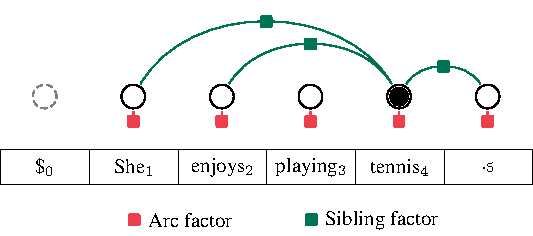
\includegraphics[scale=1]{figures/dep-factors.pdf}
        \caption{依存句法模型的因子图}
        \label{fig:con-factors}
    \end{subfigure}
    \begin{subfigure}[b]{0.8\textwidth}
        \centering
        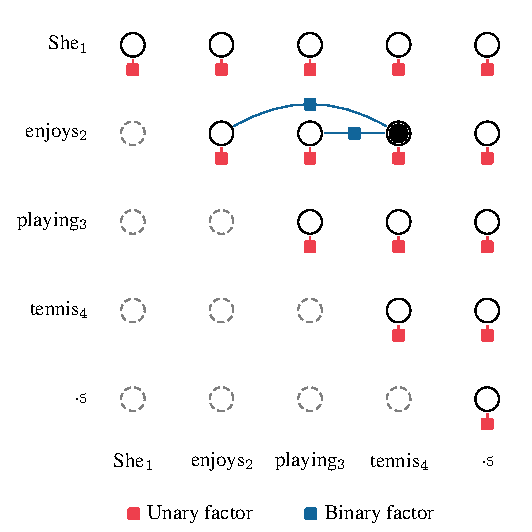
\includegraphics[scale=1]{figures/con-factors.pdf}
        \caption{成分句法模型的因子图}
        \label{fig:dep-factors}
    \end{subfigure}
    \caption{一个例句和其依存/成分句法模型对应的因子图,我们在例句上方标出了对应的正确无标签依存句法树和成分句法树,其中成分句法树进行了左二叉化.
        灰色虚线圆圈代表被屏蔽的变量.
        图中标出了所有的一阶(红色)因子,为了简洁起见,对于二阶因子,依存句法图中我们只标出了涉及弧$3\rightarrow 4$的兄弟(绿色)因子,成分句法图中只标出了和组块$(3, 4)$连接的二阶(蓝色)因子.}
    \label{fig:dep-vi-factors}
\end{figure}

\subsection{变分推断}

在得到分值之后,我们的句法分析方法分为两阶段:1)构建无标签树;2)预测标签.
在第二阶段预测标签的时候,我们以贪婪的方式给依存树的每条弧(见章节~\ref{sub@sec:dep-crf-labeling})或者成分树的每个组块(见章节~\ref{sub@sec:con-crf-model-definition})打上标签.
而在第一阶段构建无标签树时,我们的目的是选择后验概率最大的句法树$\hat{\boldsymbol{y}} = \arg\max_{\boldsymbol{y}} P(\boldsymbol{y}\mid \boldsymbol{x})$.
通常这样的推断的复杂度较高,以至于无法计算.
在句法分析领域我们可以应用Inside算法来进行精确计算,但是仍然十分影响计算效率.
因此在本节我们提出利用基于平均场理论的变分推断法来近似得到后验概率.
平均场变分推断假设句法树$\boldsymbol{y}$每个位置的变量相互独立,因此可以在线性时间内通过迭代的方法得到后验概率的近似值$Q(\boldsymbol{y})$.

关于平均场变分推断的通用更新公式以及相关推导见附录~\ref{appendix:mfvi-derivation}.
根据依存句法和成分句法任务目标的不同,我们在下面下面两小节详细阐述了通用公式针对具体任务的特化版本,以及相关的势函数(potential function)和因子图(factor graph)的设计.

\noindent\textbf{基于头选择的变分推断.}
依存句法模型的因子图见图~\ref{fig:dep-factors}

\noindent\textbf{基于二分类的变分推断.}
成分句法模型的因子图见图~\ref{fig:con-factors}

\subsection{训练}

\subsection{解码}

\subsection{复杂度分析}


\begin{figure}[tb]
    \centering
    \begin{subfigure}[b]{0.9\textwidth}
        \centering
        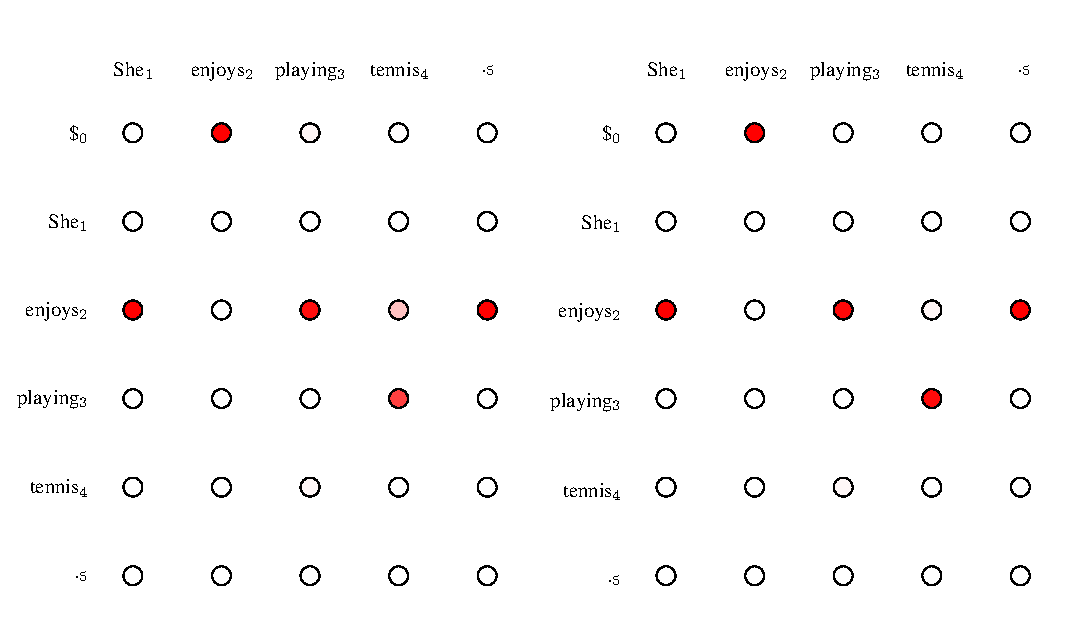
\includegraphics[scale=0.75]{figures/dep-probs.pdf}
        \caption{成分句法树每个位置对应的分值和后验概率}
        \label{fig:con-factors}
    \end{subfigure}
    \begin{subfigure}[b]{0.9\textwidth}
        \centering
        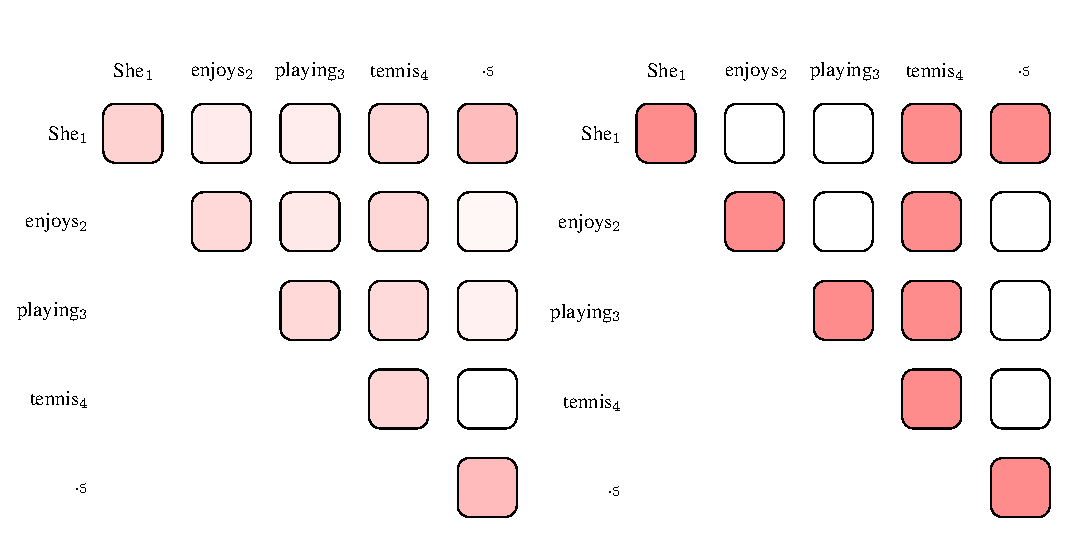
\includegraphics[scale=0.75]{figures/con-probs.pdf}
        \caption{成分句法树每个位置对应的分值和后验概率}
        \label{fig:dep-factors}
    \end{subfigure}
    \caption{一个例句对应的依存句法模型和成分句法模型的输出. 左边的图是每个位置的分值(log potential),为了方便显示,我们首先对分值进行了归一化.
        右边的图是变分推断得到的后验概率. 灰色虚线圆圈代表被屏蔽的不合法位置,颜色的深浅反应了分值/概率的大小.}

    \label{fig:dep-vi-factors}
\end{figure}

\section{实验}\label{sec:vi-exp}

\noindent\textbf{数据.}
为了方面和章节~\ref{cha:dep-crf}提出的精确推断的高阶模型进行比较,我们主要在英文的PTB和中文的CNLL09上进行了依存句法的实验.
同样的,我们在英文的PTB,中文的CTB51以及CTB7进行了成分句法分析实验.
实验数据的详细设置在章节~\ref{cha:dep-crf}和章节~\ref{cha:con-crf}有详细的设置,这里简洁起见不再重复.

\noindent\textbf{评价.}
在依存句法分析上,我们主要采用了有标签和无标签附着分值(UAS/LAS)作为评价指标,英文PTB的标点被忽略.
在成分句法分析上,我们采用了惯用的区块级别的准确率、召回率和F值(P/R/F)的指标,由标准工具\texttt{EVALB}来得到.
成分句法树在训练和评价时采用的预处理和后处理行为我们保持和章节~\ref{cha:con-crf}一致.

\noindent\textbf{参数设置.}
我们保持两种句法分析模型的编码器和训练方法与前面的章节基本一致.
对于二阶模型,我们设置依存句法分析中使用的兄弟特征以及成分句法分析使用的二阶特征的MLP层输出维度为100.
我们设置变分推断的迭代次数统一为3次.
在成分句法分析中我们新加入了一个参数$\lambda$来平衡标签和无标签树的训练损失,并设置$\lambda$为0.1.

\begin{table}[tb!]
  \centering
  \begin{tabular}{lcccc}
    \toprule
             & \multicolumn{2}{c}{PTB} & \multicolumn{2}{c}{CoNLL09}                 \\
             & UAS                     & LAS                         & UAS   & LAS   \\[2pt]
    \hline
    \\[-15pt]
    Baseline & 95.72                   & 93.97                       & 88.80 & 85.86 \\[3pt]
    LBP      &                         &                             &       &       \\
    MFVI     &                         &                             &       &       \\
    \bottomrule
  \end{tabular}
  \caption{Dev数据上的结果.}
  \label{table:dev-test}
\end{table}




\subsection{分析}

\noindent\textbf{子树和完全树的结果.}

\noindent\textbf{数据量的影响.}

\noindent\textbf{迭代次数的影响.}

\subsection{样例分析}

\subsection{速度比较}

\subsection{UD的结果}

\chapter{总结与展望}

\section{总结}
得益于深度学习技术的迅速发展,以及神经网络模型的强大建模能力,近年来句法分析领域得到了长足的进步。
\citet{dozat-etal-2017-biaffine}提出的依存句法分析器Biaffine Parser作为当前最流行的句法分析器,代表了这样一个发展趋势:采用一个强大的编码器,结合一个简单的训练目标。
本文将Biaffine Parser作为依存句法和成分句法分析两个任务的骨干架构,探索了进一步提升句法分析模型的途径。

首先,与现有方法采用的局部损失函数或者Max Margin训练方法不同,本文采用了TreeCRF作为主要的推断方法,在训练时寻求最大化句法树的概率。
一方面TreeCRF考虑到了全局树约束,带来了更好的性能。
另一方面,TreeCRF可以显式获得树和子树的概率,对于下游任务而言更加有用。
为了解决TreeCRF带来的低效问题,本文分别采用了:1)批次化Inside算法;2)高效的反向传播机制代替Outside算法;这两项技术来加速。

其次,考虑到在前人方法中采用高阶特征能够带来显著的提升。
本文在一阶模型的基础上提出了一个二阶TreeCRF的扩展,并采用了一个新颖的Triaffine结构来为二阶子树打分。
在两种句法分析任务上的结果表明,二阶TreeCRF都明显超越了一阶基于局部训练目标的模型。

二阶TreeCRF进一步增加了推断算法的复杂度,因此本文还提出利用基于平均场变分推断的近似算法代替二阶TreeCRF。
变分推断方法和二阶TreeCRF采用了相同的高阶子树特征,但是显著降低了复杂度。
在多个数据集上的结果表明,变分推断方法显著超越了一阶模型的结果,并且速度相比于二阶方法要大大提升。

总的来说,本文的主要内容如下:
\begin{enumerate}
	\item 基于TreeCRF的高阶依存句法分析\\
	      \indent 本文以当前最佳的神经依存句法分析模型Biaffine Parser为基础,提出了一个二阶TreeCRF的扩展。
	      对于二阶子树,本文提出了一个新颖的Triaffine结构来打分。
	      为了解决TreeCRF低效的问题,我们提出对于$O(n^3)$复杂的Inside算法进行批次化,利用GPU并行计算的能力将算法复杂度降低到了$O(n^2)$。
	      此外我们将复杂的Outside过程用基于自动求导机制的高效反向传播。
	      我们的加速方法让二阶模型的解析速度达到400句每秒,相比于传统在CPU上运算的方式有数十倍的提升,并且没有明显慢于一阶模型。
	      我们在13个语言的27个数据集上进行了大量的分析和实验,发现二阶模型带来了显著的准确率提升,并且尤其在全局指标,以及局部标注数据上表现良好。
	\item 基于TreeCRF的高阶成分句法分析\\
	      \indent 本文提出在已有神经网络模型的基础上应用高阶TreeCRF到成分句法分析中。
	      为了解决高复杂度问题,我们采用了和依存句法中一致的加速策略,将训练和解码算法进行了高度批次化,并且用支持自动求导机制的反向传播传播算法代替了复杂的Outside算法,从而显著提升了解析速度。
	      此外,我们提出了简单的两阶段解析方法,比前人的一阶段解析更加高效,并且没有损害性能。
	      为了提升解析效果,我们参考依存句法分析对模型架构进行了修改。
	      我们提出用双仿射打分机制代替前人的minus feature方法,并且发现在双向LSTM编码器中引入的一些诸如Dropout的参数修改可以极大提升解析的性能,达到不输于Transformer的效果。
	      在中英文的三个基准数据集上的实验结果表明,我们提出的一阶和二阶成分句法模型显著超越了前人的方法。
	      速度方面,一阶和二阶模型分别可以解析1,000和598句每秒。
	      在使用BERT之后,我们的模型在大部分数据集上都达到了新的最佳结果。
	\item 基于变分推断的高效句法分析方法\\
	      \indent 考虑到精确推断的TreeCRF方法的高复杂度问题,本文中我们将包含二阶特征的平均场变分推断引入到了依存句法和成分句法分析中,使得算法在GPU上的复杂度从$O(n^2)$降低到了$O(n)$。
	      根据两种句法分析任务的不同学习特性,我们采取了不同的变分推断更新策略,在依存句法分析上我们采取了一个包含头选择约束的更新方法,在成分句法分析上我们则引入了一个基于二分类学习目标的更新方法。
	      我们在中英文共五个数据集上做了实验,结果表明我们的方法显著超越了采用局部学习目标的方法,并达到了和精确推断的二阶TreeCRF方法可比较的性能。
	      在使用BERT之后,变分推断方法在所有数据上都达到或接近了现有模型的最佳水平。
\end{enumerate}

\section{未来展望}
本文在依存句法和成分句法分析两个任务上分别尝试了基于树形随机场的融入高阶特征的结构化学习方法,让句法分析模型达到了新的最佳水平。
本文还尝试了应用基于变分推断的近似推断算法,显著降低了高阶TreeCRF的复杂度,大大提升了句法分析速度。
未来,本文打算基于已有成果从一下几个方面继续探索:
\begin{enumerate}
	\item 本文的句法分析模型主要采用了3层双向LSTM作为编码器。
	      考虑到Transformer的迅速发展,以及BERT预训练语言模型的强大作用,未来我们将尝试利用Transformer替换已有编码器,探讨自注意力机制的效果,以及语言模型不同的利用方式,例如特征集成和微调对模型性能的影响。
	\item 本文中为了方便起见我们只采用了一种高阶特征,例如依存模型中我们只采用了邻接兄弟特征,成分模型中采用了区块分割点特征。
	      在未来我们将尝试更多的特征设计,探讨他们对模型效果的影响。
	\item 在本文中我们只尝试了基于平均场变分推断的近似推断算法。
	      然而,仍然有其他的近似算法在NLP社区有广泛的应用,例如循环置信传播、对偶分解、整数线性规划等等。
	      在未来我们打算尝试更多近似算法,并对他们做一些经验性比较。
\end{enumerate}


% % 参考文献,4或者小4楷体
% !Mode:: "TeX:UTF-8"
%\cleardoublepage

\addcontentsline{toc}{chapter}{参考文献}
% \nocite{*}
\begin{kai}
    \bibliography{thesis}
\end{kai}
% \cleardoublepage


% % 附录,4或者小4楷体
% \begin{appendix}
% \chapter{CTB到PD的宽松映射}

\setlength{\tabcolsep}{5pt}
% \begin{table}                   %table 环境是一个表格浮动环境, [htbp]控制插入位置,h当前位置,t顶部,b底部,p独立页
% \begin{small}
% \begin{center}
\begin{kai}
    %\vspace{0.5em}%\centering%\xiaowuhao      %定义表中数据的尺寸
    % \centering
    \begin{longtable}{p{0.9cm} p{2.8cm} p{3cm} p{0.5\columnwidth}}                    %c表示居中,l表示左对齐,r表示右对齐
        词性 & 名称           & 示例                   & 对应的PD词性                                                                                                                                                                                       \\
        AD   & 副词           & 不\quad 也\quad 就     & Ag\quad Dg\quad Tg\quad Vg\quad a\quad ad\quad b\quad c\quad d\quad f\quad h\quad i\quad j\quad l\quad m\quad n\quad q\quad r\quad s\quad t\quad v\quad vd\quad vn\quad z                          \\
        AS   & 动态助词       & 了\quad 著\quad 过     & u\quad y                                                                                                                                                                                           \\
        BA   & 把字结构       & 将\quad 把             & p                                                                                                                                                                                                  \\
        CC   & 并列连接词     & 和\quad 与\quad        & c\quad d\quad p\quad v                                                                                                                                                                             \\
        CD   & 限定数量词     & 一\quad 两\quad 三     & a\quad m\quad q\quad r                                                                                                                                                                             \\
        CS   & 从属连接词     & 虽然\quad 如果\quad 若 & Dg\quad c\quad d\quad p                                                                                                                                                                            \\
        DEC  & 补语或名词化   & 的\quad 之             & u                                                                                                                                                                                                  \\
        DEG  & 关联或所有格   & 的\quad 之             & u                                                                                                                                                                                                  \\
        DER  & 补语短语``得'' & 得                     & u                                                                                                                                                                                                  \\
        DEV  & 方式``地''     & 地                     & u                                                                                                                                                                                                  \\
        DT   & 限定词         & 这\quad 各\quad 全     & Tg\quad m\quad r                                                                                                                                                                                   \\
        ETC  & 等等           & 等\quad 等等\quad      & u                                                                                                                                                                                                  \\
        FW   & 外来词         & A\quad E\quad B        & nx\quad w                                                                                                                                                                                          \\
        IJ   & 感叹词         & 唉呀\quad 哈拉         & e\quad y                                                                                                                                                                                           \\
        JJ   & 名词修饰词     & 大\quad 新\quad 小     & Ag\quad Tg\quad a\quad ad\quad an\quad b\quad d\quad f\quad h\quad i\quad j\quad l\quad m\quad n\quad q\quad r\quad s\quad t\quad v\quad vd\quad vn\quad z                                         \\
        LB   & 长``被''结构   & 被\quad 为\quad 受     & p\quad v                                                                                                                                                                                           \\
        LC   & 方位词         & 中\quad 上\quad 时     & Ng\quad Tg\quad f\quad m\quad u\quad v                                                                                                                                                             \\
        M    & 量词           & 个\quad 年\quad 美元   & Ng\quad n\quad p\quad q                                                                                                                                                                            \\
        MSP  & 其他助词       & 所\quad 而\quad 来     & c\quad u\quad v                                                                                                                                                                                    \\
        NN   & 名词           & 经济\quad 企业\quad 人 & Ag\quad Ng\quad Vg\quad a\quad ad\quad an\quad b\quad c\quad f\quad i\quad j\quad k\quad l\quad m\quad n\quad nr\quad nt\quad nx\quad nz\quad q\quad r\quad s\quad t\quad v\quad vd\quad vn\quad z \\
        NR   & 专有名词       & 中国\quad 台湾         & Ng\quad f\quad j\quad m\quad n\quad nr\quad ns\quad nt\quad nz\quad t                                                                                                                              \\
        NT   & 时间名词       & 目前\quad 去年         & Tg\quad d\quad m\quad q\quad r\quad t                                                                                                                                                              \\
        OD   & 数词           & 第一\quad 第二\quad 首 & m                                                                                                                                                                                                  \\
        ON   & 拟声词         & o                                                                                                                                                                                                                           \\
        P    & 介词           & 在\quad 对\quad 以     & p\quad v                                                                                                                                                                                           \\
        PN   & 代词           & 他\quad 我\quad 自己   & n\quad q\quad r\quad u                                                                                                                                                                             \\
        PU   & 标点符号       & ,\quad . \quad \quad  & w                                                                                                                                                                                                  \\
        SB   & 短``被''结构   & 被\quad 遭             & p                                                                                                                                                                                                  \\
        SP   & 句末助词       & 了\quad 的\quad 吗     & u\quad y                                                                                                                                                                                           \\
        VA   & 谓词性形容词   & 大\quad 多\quad 好     & Ag\quad Vg\quad a\quad ad\quad an\quad b\quad i\quad l\quad m\quad n\quad r\quad v\quad vd\quad vn\quad z                                                                                          \\
        VC   & 系动词         & 是\quad 为\quad 非     & Vg\quad v                                                                                                                                                                                          \\
        VE   & 主要动词``有'' & 有\quad 没有\quad 无   & v                                                                                                                                                                                                  \\
        VV   & 动词           & 说\quad 要\quad 会     & Ag\quad Ng\quad Vg\quad a\quad c\quad d\quad f\quad i\quad j\quad l\quad n\quad p\quad r\quad u\quad v\quad vd\quad vn                                                                             \\
        
        % \toprule[1pt]                           %绘制表格最顶部的水平线
        % \midrule[1pt]                           %绘制表头下的水平线
        % \bottomrule[1pt]                        %绘制表格最底部的水平线
    \end{longtable}
\end{kai}
% \end{center}
% \caption{Summary of the Peking University Part-of-speech Tagset.}
% \end{small}
% \end{table}
% \chapter{PD到CTB的宽松映射}

% \setlength{\tabcolsep}{5pt}
% \begin{table}\quad    %table 环境是一个表格浮动环境, [htbp]控制插入位置,h当前位置,t顶部,b底部,p独立页
% \begin{small}
% \begin{center}
\begin{kai}
    %\vspace{0.5em}%\centering%\xiaowuhao\quad   %定义表中数据的尺寸
    % \centering
    \begin{longtable}{p{0.9cm} p{1.7cm} p{3.9cm} p{0.5\columnwidth}}
        词性 & 名称     & 示例                     & 对应的CTB词性                                                                              \\
        Ag   & 形容词素 & 优\quad 奇\quad 廉       & NN\quad VA\quad AD\quad VV\quad JJ                                                         \\
        Dg   & 副词素   & 甚\quad 俱\quad 复       & AD\quad CS                                                                                 \\
        Ng   & 名语素   & 时\quad 讯\quad 民       & NN\quad LC\quad VV\quad M\quad NR                                                          \\
        Tg   & 时语素   & 现\quad 晚\quad 今       & NT\quad JJ\quad AD\quad DT\quad LC                                                         \\
        Vg   & 动语素   & 摄\quad 创\quad 具       & VV\quad NN\quad AD\quad VA\quad VC                                                         \\
        a    & 形容词   & 大\quad 新\quad 好       & VA\quad JJ\quad AD\quad NN\quad VV\quad CD                                                 \\
        ad   & 副形词   & 积极\quad 全面\quad 认真 & AD\quad JJ\quad NN\quad VA                                                                 \\
        an   & 名形词   & 安全\quad 困难\quad 努力 & NN\quad VA\quad JJ                                                                         \\
        b    & 区别词   & 副\quad 主要\quad 女     & JJ\quad NN\quad VA\quad AD                                                                 \\
        c    & 连词     & 和\quad 而\quad 并       & CC\quad CS\quad MSP\quad AD\quad VV\quad NN                                                \\
        d    & 副词     & 不\quad 也\quad 就       & AD\quad JJ\quad VV\quad NT\quad CC\quad CS                                                 \\
        e    & 叹词     & 嗬\quad 啊\quad 哦       & IJ                                                                                         \\\\
        f    & 方位词   & 中\quad 上\quad 后       & LC\quad NN\quad JJ\quad VV\quad AD\quad NR                                                 \\
        h    & 前接成分 & 非\quad 超\quad 准       & AD\quad JJ                                                                                 \\
        i    & 成语     & 实事求是\quad 艰苦奋斗   & VV\quad NN\quad VA\quad AD\quad JJ                                                         \\
        j    & 间称略词 & 中\quad 美\quad 人大     & NR\quad NN\quad JJ\quad VV\quad AD                                                         \\
        k    & 后接成分 & 们\quad 者\quad 式       & NN                                                                                         \\
        l    & 习用语   & 近年来\quad 发展中国家   & VV\quad NN\quad AD\quad VA\quad JJ                                                         \\
        m    & 数词     & 一\quad 两\quad 一个     & CD\quad OD\quad AD\quad DT\quad NT\quad NN\quad LC\quad NR\quad JJ\quad VA                 \\
        n    & 名词     & 人\quad 经济\quad 企业   & NN\quad JJ\quad NR\quad VV\quad M\quad VA\quad AD\quad PN                                  \\
        nr   & 人名     & 周恩来\quad 邓小平       & NR\quad NN                                                                                 \\
        ns   & 地名     & 中国\quad 北京\quad 美国 & NR                                                                                         \\
        nt   & 机构团体 & 国务院\quad 联合国       & NR\quad NN                                                                                 \\
        nx   & 非汉字串 & A\quad VCD\quad B   & NN\quad FW                                                                                 \\
        nz   & 其他专名 & 中华\quad 汉族           & NR\quad NN                                                                                 \\
        o    & 拟声词   & 隆隆\quad 汩汩\quad 潺潺 & ON                                                                                         \\
        p    & 介词     & 在\quad 对\quad 为       & P\quad VV\quad LB\quad CC\quad CS\quad SB\quad M\quad BA                                   \\
        q    & 量词     & 个\quad 年\quad 次       & M\quad NN\quad AD\quad CD\quad JJ\quad NT\quad PN                                          \\
        r    & 代词     & 这\quad 他\quad 我们     & PN\quad DT\quad NN\quad AD\quad JJ\quad CD\quad VA\quad NT\quad VV                         \\
        s    & 处所词   & 国内\quad 当地\quad 一起 & NN\quad JJ\quad AD                                                                         \\
        t    & 时间词   & 今天\quad 今年\quad 目前 & NT\quad NN\quad AD\quad NR\quad JJ                                                         \\
        u    & 助词     & 的\quad 了\quad 等       & DEC\quad DEG\quad ETC\quad AS\quad DER\quad MSP\quad DEV\quad LC\quad PN\quad VV\quad SP   \\
        v    & 动词     & 是\quad 有\quad 要       & VV\quad NN\quad P\quad AD\quad VE\quad VA\quad JJ\quad VC\quad MSP\quad CC\quad LC\quad LB \\
        vd   & 副动词   & 持续\quad 优先\quad 综合 & AD\quad VV\quad NN\quad JJ\quad VA                                                         \\
        vn   & 名动词   & 工作\quad 发展\quad 建设 & NN\quad JJ\quad VV\quad AD\quad VA                                                         \\
        w    & 标点符号 & ,\quad . \quad 、       & PU\quad FW                                                                                 \\
        y    & 语气词   & 了\quad 呢\quad 吗       & SP\quad AS\quad IJ                                                                         \\
        z    & 状态词   & 优良\quad 最佳\quad 短短 & VA\quad JJ\quad NN\quad AD                                                                 \\
        % \toprule[1pt]\quad    %绘制表格最顶部的水平线
        % \midrule[1pt]\quad    %绘制表头下的水平线
        % \bottomrule[1pt]\quad %绘制表格最底部的水平线
    \end{longtable}
\end{kai}
% \end{center}
% \caption{Summary of the Peking University Part-of-speech Tagset.}
% \end{small}
% \end{table}
% \end{appendix}

% 附页标题样式
\backmatter
% 附页
\chapter{攻读学位期间的成果}

\begin{itemize}
	\setlength{\itemsep}{5pt}
	% \setlength{\parsep}{2em}
	
	\item \textbf{\heiti\sihao{论文}}
	      \begin{enumerate}
	      	\setlength{\itemsep}{-\itemsep}  %调整间距
	      	% \usecounter{numcount} % 使用计数器,初始值为0
	      	% \setlength{\leftmargin}{3em} %左边界
	      	% \setlength{\parsep}{-0.5ex} %段落间距
	      	% \setlength{\topsep}{-10ex} %列表到上下文的垂直距离
	      	% \setlength{\itemsep}{0.5ex} %条目间距
	      	% \setlength{\labelsep}{0.3em} %标号和列表项之间的距离,默认0.5em
	      	% \setlength{\itemindent}{1.1em} %标签缩进量
	      	% \setlength{\listparindent}{0em} %段落缩进量
	      	
	      	\item Annual Meeting of the Association for Computational Linguistics (ACL, CCF-A会议). 2020. 一作. 已录用
	      	\item International Joint Conference on Artificial Intelligence (IJCAI, CCF-A会议). 2020. 一作. 已录用
	      	\item Natural Language Processing and Chinese Computing (NLPCC, CCF-C会议). 2020. 共同一作. 已录用
	      	\item International Workshop on Semantic Evaluation (SemEval). 2019. 三作. 已录用
	      	      
	      \end{enumerate}
	      
	\item \textbf{\heiti\sihao{比赛}}
	      \begin{enumerate}
	      	\item *2020语言与智能技术竞赛比赛,第六名.
	      	\item *2019语义分析国际评测比赛,第一名.
	      \end{enumerate}
	      
	\item \textbf{\heiti\sihao{实习}}
	      \begin{enumerate}
	      	\item \textsc{2020/8--2021/2}. 杭州-阿里巴巴-达摩院.
	      \end{enumerate}
	      
\end{itemize}

\chapter{致谢}

养天地正气,法古今完人.
从本科到硕士,转眼间在美丽的苏州大学校园内度过了七年的求学时光.
在这段不算短的人生旅途中,无论是学识上还是生活阅历上我都成长良多.

首先,我要感谢我的导师李正华老师.
李老师永远以饱满的热情和专注的态度面对工作和生活,永远是我以后希望成为一个独立研究者的榜样.

感谢尊敬的张民老师,张老师以高标准要求每一个学生,营造了组内专一浓厚的科研氛围.
此外,张老师敏锐的思维、渊博的知识、平易近人的风格、深深的影响了我,平时的相处让我获益良多.
感谢陈文亮老师,陈老师开朗热情,在学业上也给予了我很多指导.

同样感谢周国栋、朱巧明、李寿山、洪宇和李军辉等苏州大学自然语言处理实验室的所有老师,各位老师严谨的治学态度和进取的专业精神是我的榜样.

感谢同组的夏庆荣师兄、龚晨师姐、李英师姐和张月师姐,各位师兄师姐总是十分热心的解决我生活和研究上遇到的困难.
感谢章波、黄德朋、江心舟师兄,彭雪师姐,在我还是萌新的时候对我的帮助,以及平时对我的关照.
感谢同届的同学蒋炜、陆凯华、吴锟、刘亚慧,大家在一起互相帮助,互相进步.
感谢周厚全、沈嘉钰、李嘉诚、侯洋、李帅克、周仕林、刘泽洋、李扬师弟,还有周明月、杨浩萍师妹,十分珍惜与大家相处的美好时光.
此外,还要感谢实习期间相处的蒋勇师兄以及王新宇同学,特别是感谢蒋勇师兄在我实习期间对我的关照,以及在课题研究上的悉心帮助和指导.

感谢我的父母还有家人们,你们总是我心灵上的港湾和寄托,无论何时都能给我最无私的帮助.

最后,我还要感谢各位评审老师,感谢各位老师们在百忙之中抽取时间对本文进行评审,并提出宝贵的修改意见.



\end{document}
